\documentclass[ignorenonframetext,xcolor=x11names]{beamer}

\definecolor{mun}{RGB}{134,38,51}
\definecolor{mun2}{RGB}{99,102,106}
%\definecolor{mun}{cmyk}{0,.3922,.2392,.1686}
\definecolor{code}{RGB}{0, 0, 128}
\definecolor{code}{gray}{0.95}

\mode<presentation>
{
%  \usetheme{boxes}
%  \usetheme{default}
%  \usetheme{Montpellier}
%  \usetheme{Singapore}
%   \usetheme{Rochester}
%  \usecolortheme{crane}
%  \usecolortheme{dolphin}
%  \usecolortheme{lily}
%  \usecolortheme{orchid}
  \usecolortheme{rose}
  \setbeamercovered{transparent}
%  \usefonttheme[onlymath]{serif}
  \setbeamercolor*{structure}{bg=mun,fg=mun}
  \setbeamercolor*{palette primary}{use=structure,fg=white,bg=structure.fg}
  \setbeamercolor*{palette secondary}{use=structure,fg=white,bg=structure.fg}
  \setbeamercolor*{palette tertiary}{use=structure,fg=white,bg=black}
  \setbeamercolor*{palette quaternary}{fg=white,bg=black}
  \setbeamercolor{section in toc}{fg=black,bg=white}
  \setbeamercolor{alerted text}{use=structure,fg=structure.fg!50!black!80!black}
  \setbeamercolor{titlelike}{parent=palette primary,fg=structure.fg!50!black}
  \setbeamercolor{frametitle}{bg=mun,fg=white}
  \setbeamercolor*{titlelike}{parent=palette primary}

  \setbeamercolor{normal text}{fg=black!90}
  \setbeamercolor{math text}{fg=black}
  \setbeamercolor{quote}{bg=gray!20}
  \setbeamercolor{quotation}{bg=gray!20}
  \setbeamerfont{cite}{size=\scriptsize}
  \setbeamerfont{quote}{size=\footnotesize}
  \setbeamerfont{quotation}{size=\footnotesize}
  \setbeamercolor{red text}{fg=red!75!black}
  \setbeamertemplate{bibliography item}[triangle]
  \setbeamertemplate{enumerate item}[square]
  \setbeamertemplate{blocks}[rounded][shadow=true]
  \setbeamertemplate{navigation symbols}{}
  \setbeamertemplate{footline}[frame number]
}
\usepackage{tcolorbox}
\usepackage{amsmath}
\usepackage{physics}
\usepackage{pgf}
\usepackage[english]{babel}
\usepackage[latin1]{inputenc}
\usepackage{times}
\usepackage[T1]{fontenc}
\usepackage{multicol}
\usepackage{multirow}
\usepackage{fancyvrb}
\usepackage{tabularx}
\usepackage{amsmath}
\usepackage{bbm}
\usepackage{alltt}
\usepackage{hyperref}
\hypersetup{
    colorlinks=true,
    linkcolor=blue,
    filecolor=magenta,      
    urlcolor=blue,
}
\usepackage{minted}
\newminted{cypher}{autogobble,bgcolor=code,breakbytoken,frame=single,framesep=3pt}
\newminted{R}{autogobble,bgcolor=code,breakbytoken,frame=single,framesep=3pt}
\newminted{text}{autogobble,bgcolor=code,breakbytoken,frame=single,framesep=3pt}
\newminted{sql}{autogobble,bgcolor=code,breakbytoken,frame=single,framesep=3pt}
\newminted{bash}{autogobble,bgcolor=code,breakbytoken,python3,frame=single,framesep=3pt}
\newminted{xml}{autogobble,bgcolor=code,breakbytoken,python3,frame=single,framesep=3pt}
\newminted{python}{bgcolor=code,breakbytoken,python3,frame=single,framesep=3pt}
\newminted{html}{autogobble,bgcolor=code,breakbytoken,frame=single,framesep=3pt}
\newminted{js}{autogobble,bgcolor=code,breakbytoken,frame=single,framesep=3pt}
\AtBeginEnvironment{minted}{%
  \renewcommand{\fcolorbox}[4][]{#4} \scriptsize}
\AtEndEnvironment{minted}{%
  \normalsize}

%\newcommand{\Pr}{\operatorname{Pr}}
\newcommand{\argmax}{\operatorname*{argmax}}
\newcommand{\argmin}{\operatorname*{argmin}}
\newcommand{\Ident}{\operatorname{I}}

\author % (optional, use only with lots of authors)
{Joerg Evermann}
% - Give the names in the same order as the appear in the paper.
% - Use the \inst{?} command only if the authors have different
%   affiliation.

\institute%[Universities of Somewhere and Elsewhere] % (optional, but mostly needed)
{
  Faculty of Business Administration\\
  Memorial University of Newfoundland \\ 
  \texttt{jevermann@mun.ca} 
}

\date{}

\pgfdeclareimage[width=1.5cm]{university-logo}{../MUN_LOGO_CMYK}
\logo{\pgfuseimage{university-logo}}

% If you wish to uncover everything in a step-wise fashion, uncomment
% the following command: 

%\beamerdefaultoverlayspecification{<+->}


\title{Business 4720 - Class 15}

\subtitle{Neural Networks using Python}

\begin{document}

\begin{frame}{}
  \titlepage
  \footnotesize
  \begin{center}

\includegraphics[height=.5in]{../by-nc.png}

Unless otherwise indicated, the copyright in this material is owned by Joerg Evermann. This material is licensed to you under the \href{https://creativecommons.org/licenses/by-nc/4.0/}{Creative Commons by-attribution non-commercial license (CC BY-NC 4.0)}
\end{center}

\end{frame}

\section{Introduction}

\begin{frame}{This Class}

\begin{block}{What You Will Learn:}
\begin{itemize}
  \item Deep Learning Concepts
  \begin{itemize}
     \item Neural Network
     \item Activation Functions
     \item Gradients
     \item Backpropagation
     \item Regularization with Dropouts
 \end{itemize}
 \item Deep Learning in Python using Tensoflow
 \begin{itemize}
     \item Tensors
     \item Models
     \item Training
  \end{itemize}
\end{itemize}
\end{block}
\end{frame}

\begin{frame}{Based On}
\small
\begin{block}{}
Gareth James, Daniel Witten, Trevor Hastie and Robert Tibshirani: \emph{An Introduction to Statistical Learning with Applications in R}. 2nd edition, corrected printing, June 2023. (ISLR2) \\
\vspace{1mm}
\url{https://www.statlearning.com} \\
\vspace{1mm}
Chapter 10
\end{block}

\begin{block}{}
Kevin P. Murphy: \emph{Probabilistic Machine Learning -- An Introduction}. MIT Press 2022. \\
\vspace{1mm}
\url{https://probml.github.io/pml-book/book1.html} \\
\vspace{1mm}
Chapter 13, 14, 15
\end{block}

\begin{block}{Tensorflow Guides}
\url{https://www.tensorflow.org/guide}
\end{block}
\end{frame}

\begin{frame}{Resources}
Implementations are available on the following GitHub repo:

\url{https://github.com/jevermann/busi4720-ml} \\


The project can be cloned from this URL:

\url{https://github.com/jevermann/busi4720-ml.git}
\end{frame}

\begin{frame}{Resources}
\small

Tensorflow Playground: \url{https://playground.tensorflow.org}

\begin{center}
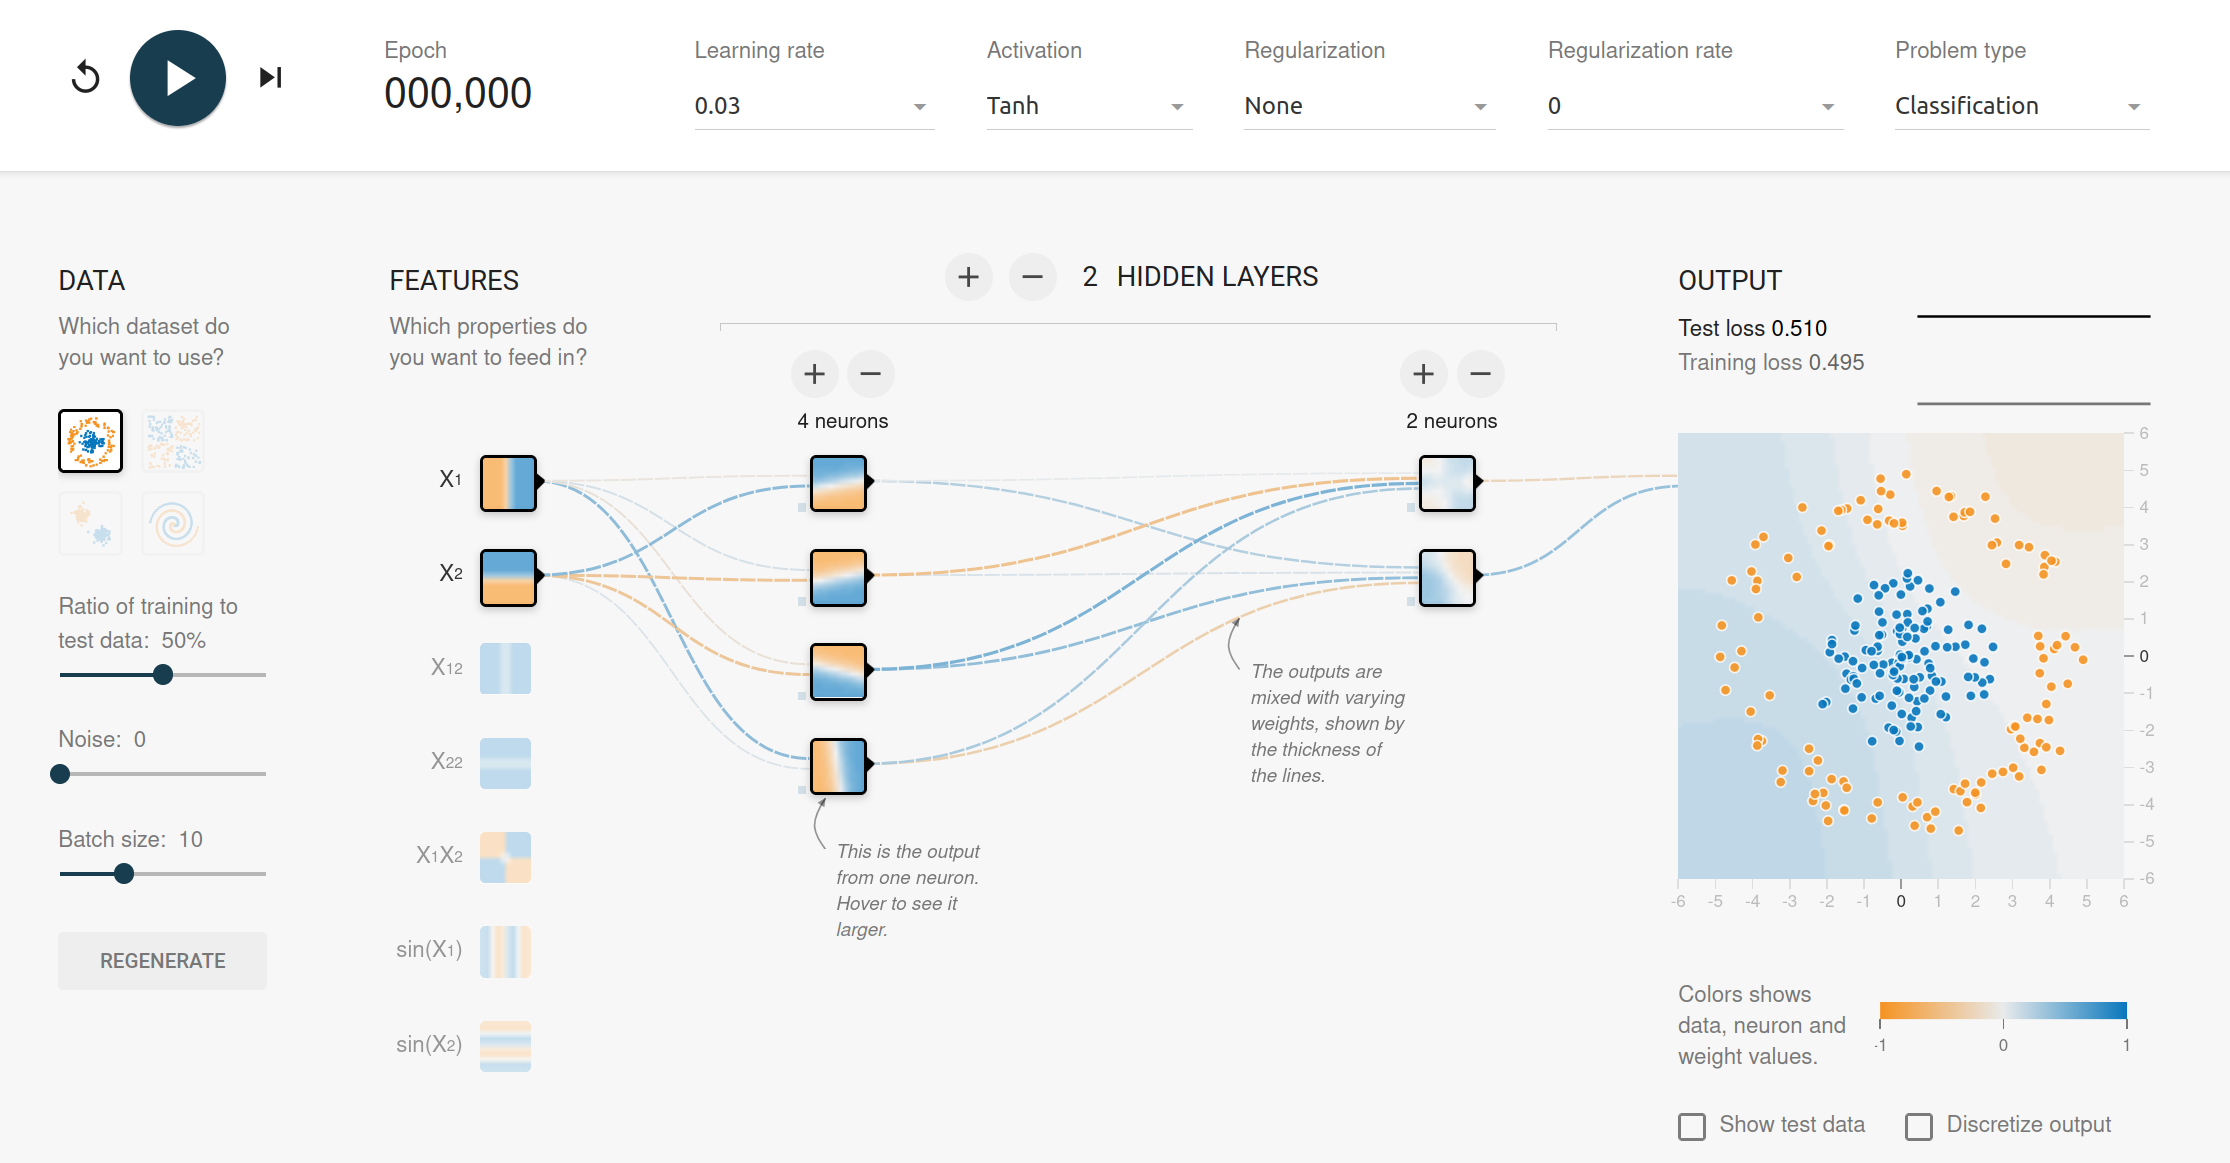
\includegraphics[width=.9\textwidth]{tensorflowplayground.png}
\end{center}


\end{frame}


\begin{frame}{Biological Neuron}
\begin{itemize}
  \item Brain cell
  \item Connected to other brain cells
  \item Receives, modulates and emits electro-chemical stimulus (''activation'')
\end{itemize}
\centering
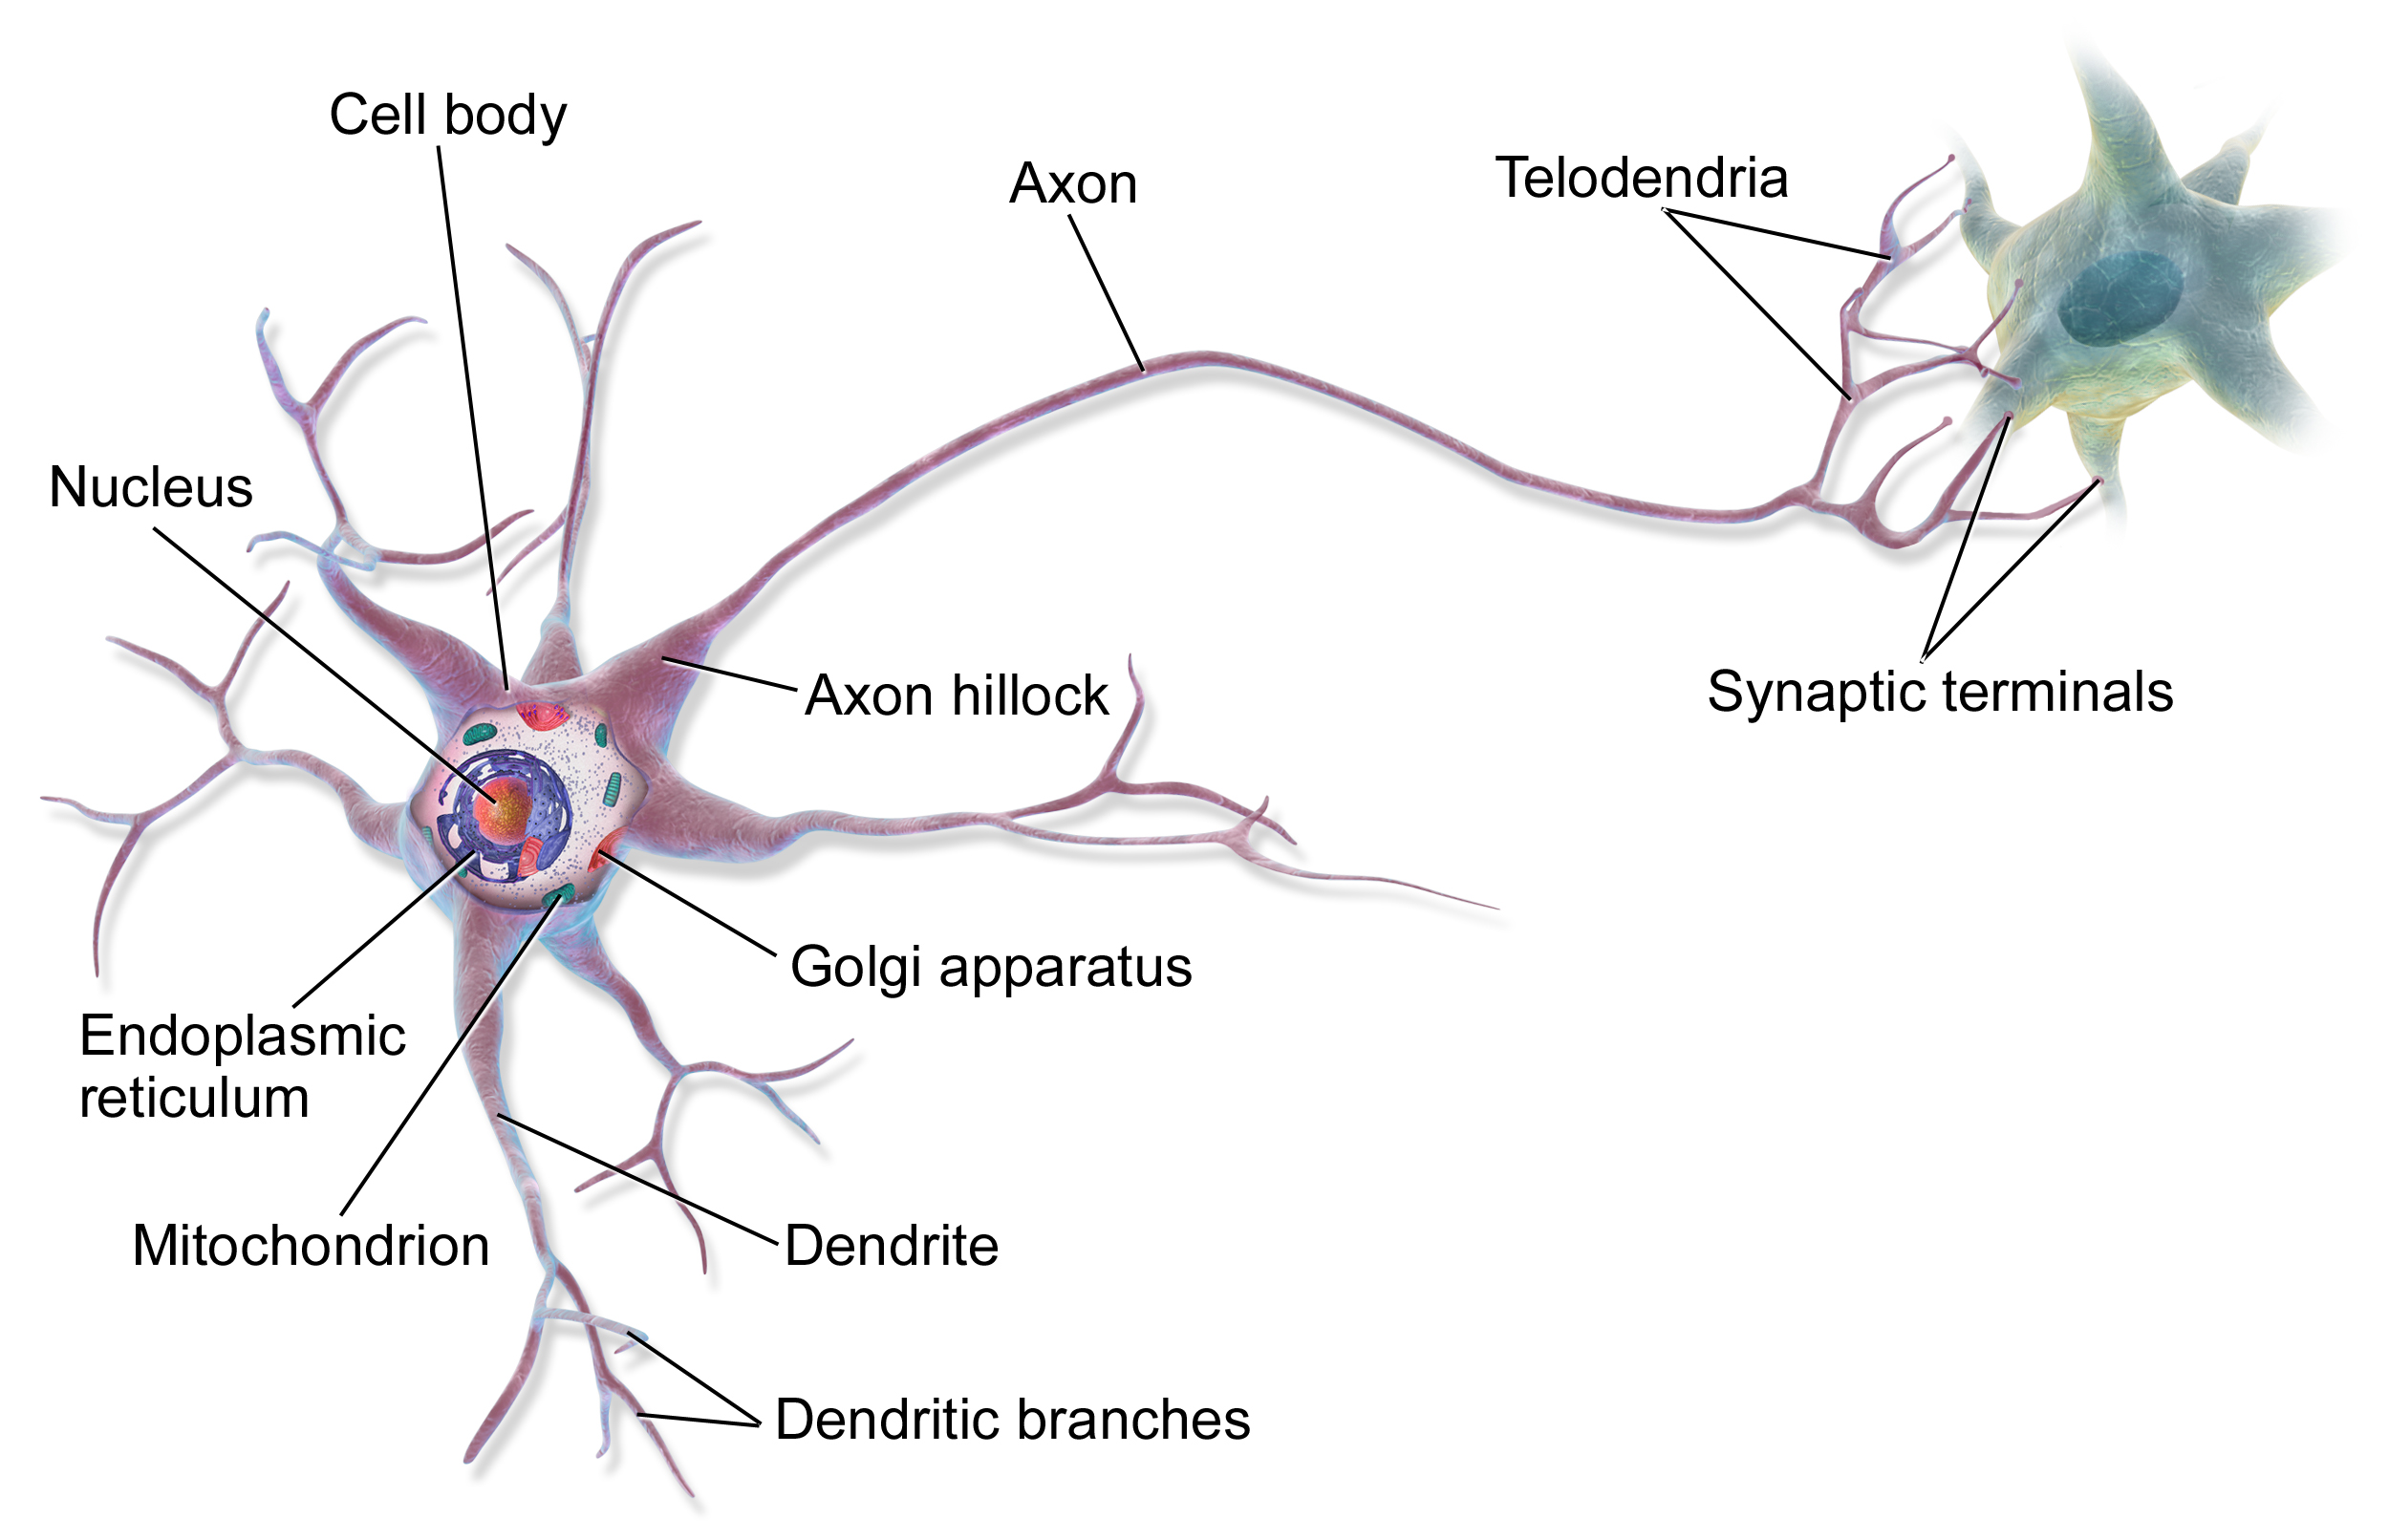
\includegraphics[width=.7\textwidth]{Blausen_0657_MultipolarNeuron.png}
\scriptsize \url{https://commons.wikimedia.org/wiki/File:Blausen_0657_MultipolarNeuron.png}
\end{frame}

\begin{frame}{Artificial Neuron}
\begin{align*}
y = \psi( b + \sum_i w_i x_i )
\end{align*}
\begin{itemize}
   \item Multiple \textbf{input} connections $x_i$
   \item Weighted using \textbf{weights} $w_i$
   \item Add a \textbf{bias} term $b$
   \item Apply \emph{nonlinear} \textbf{activation function} $\psi$
\end{itemize}
\end{frame}

%\begin{frame}{Popular Activation Functions}
%\footnotesize
%\centering
%\begin{tabular}{m{.8in}|m{1.5in}|m{1in}} \hline
%Sigmoid & $\displaystyle \frac{e^z}{1+e^z}$ & 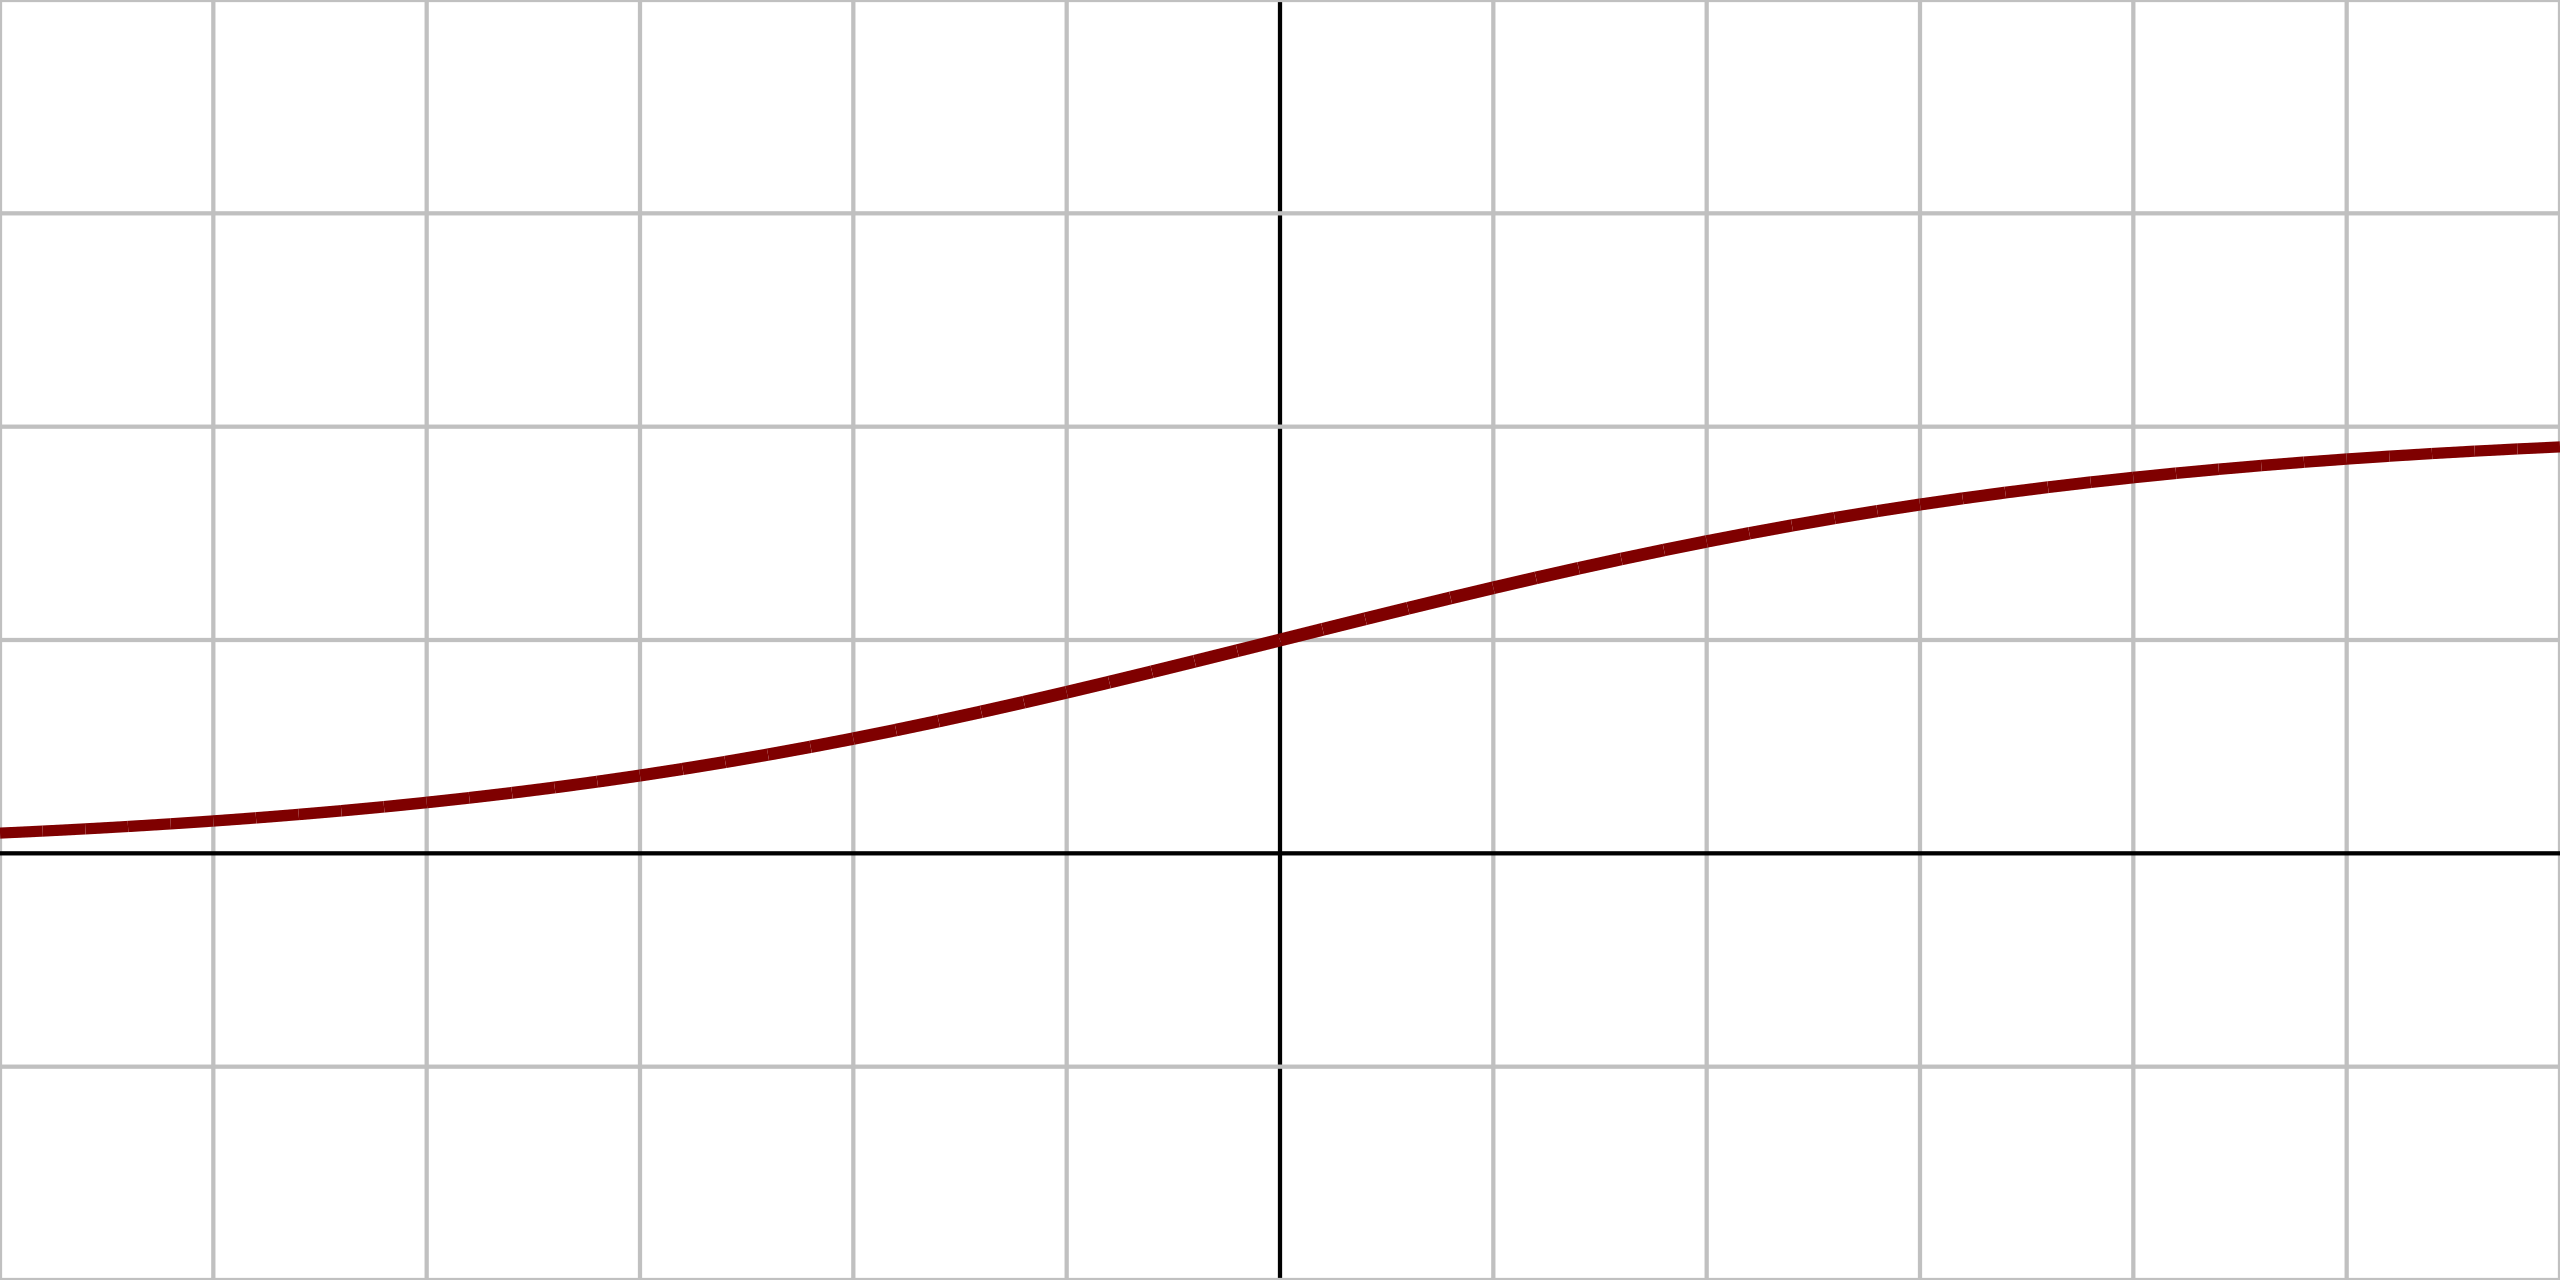
\includegraphics[width=1in]{sigmoid.png} \\ \hline
%Tanh & $\displaystyle \frac{sinh(z)}{cosh(z)} = \frac{e^z-e^{-z}}{e^z+e^{-z}}$ & 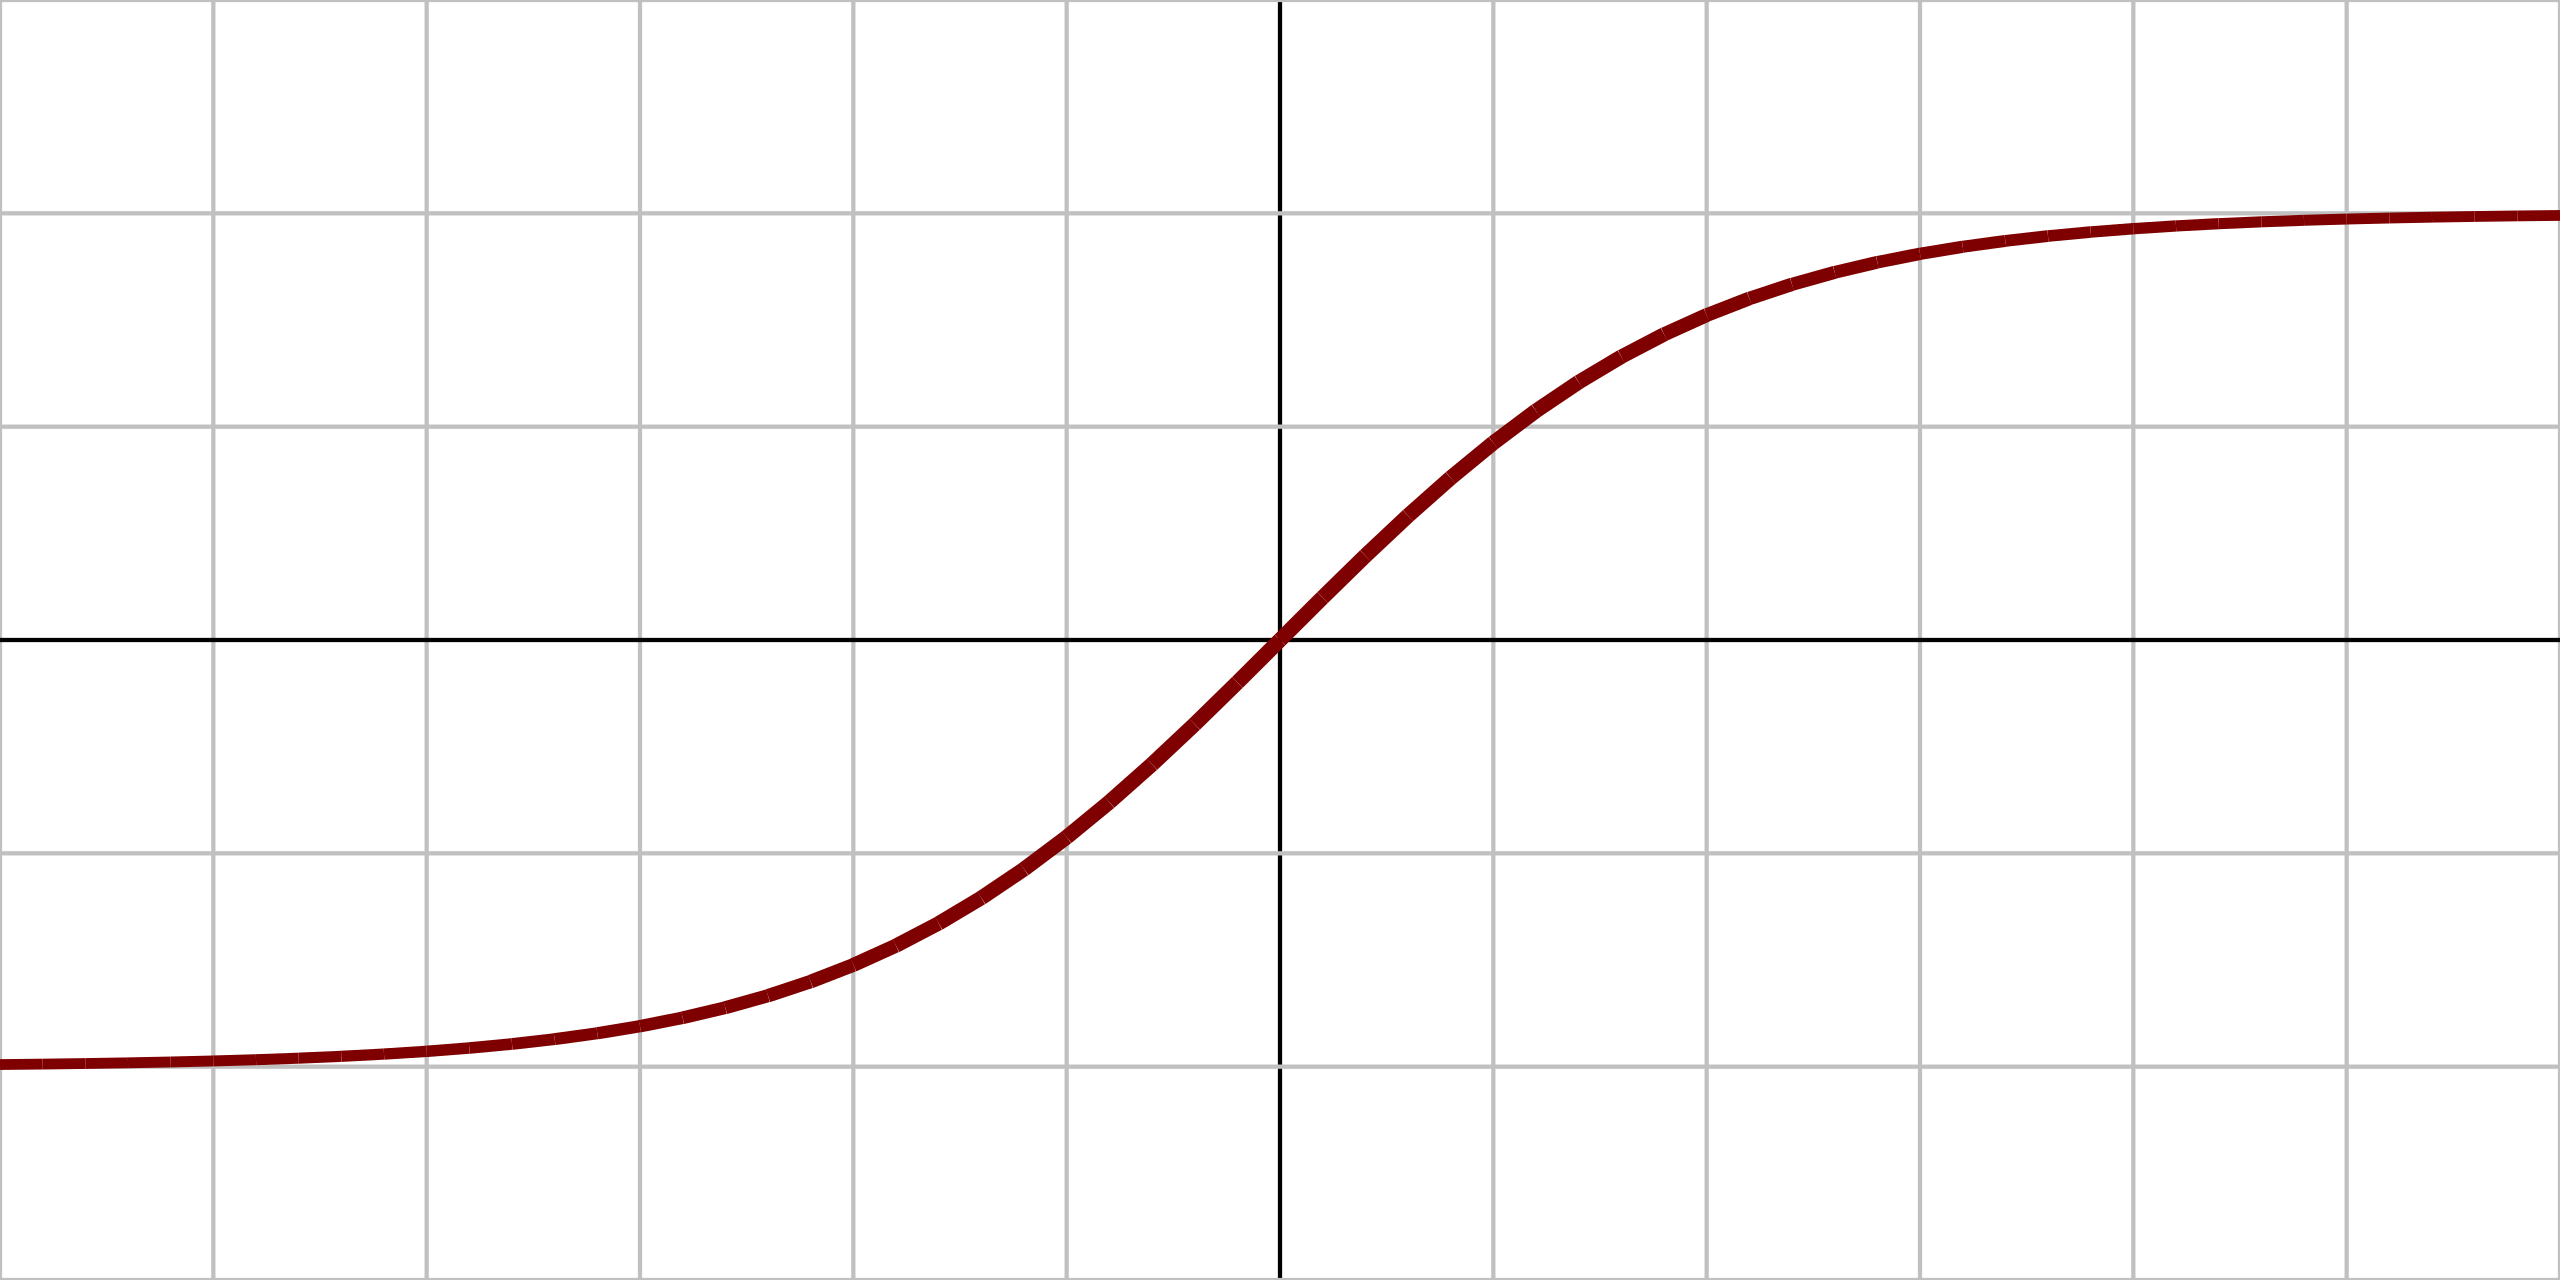
\includegraphics[width=1in]{tanh.png} \\ \hline
%ReLU & $\displaystyle \begin{cases}
%0 & \text{if} z \leq 0 \\
%z & \text{if} z > 0
%\end{cases}$ & 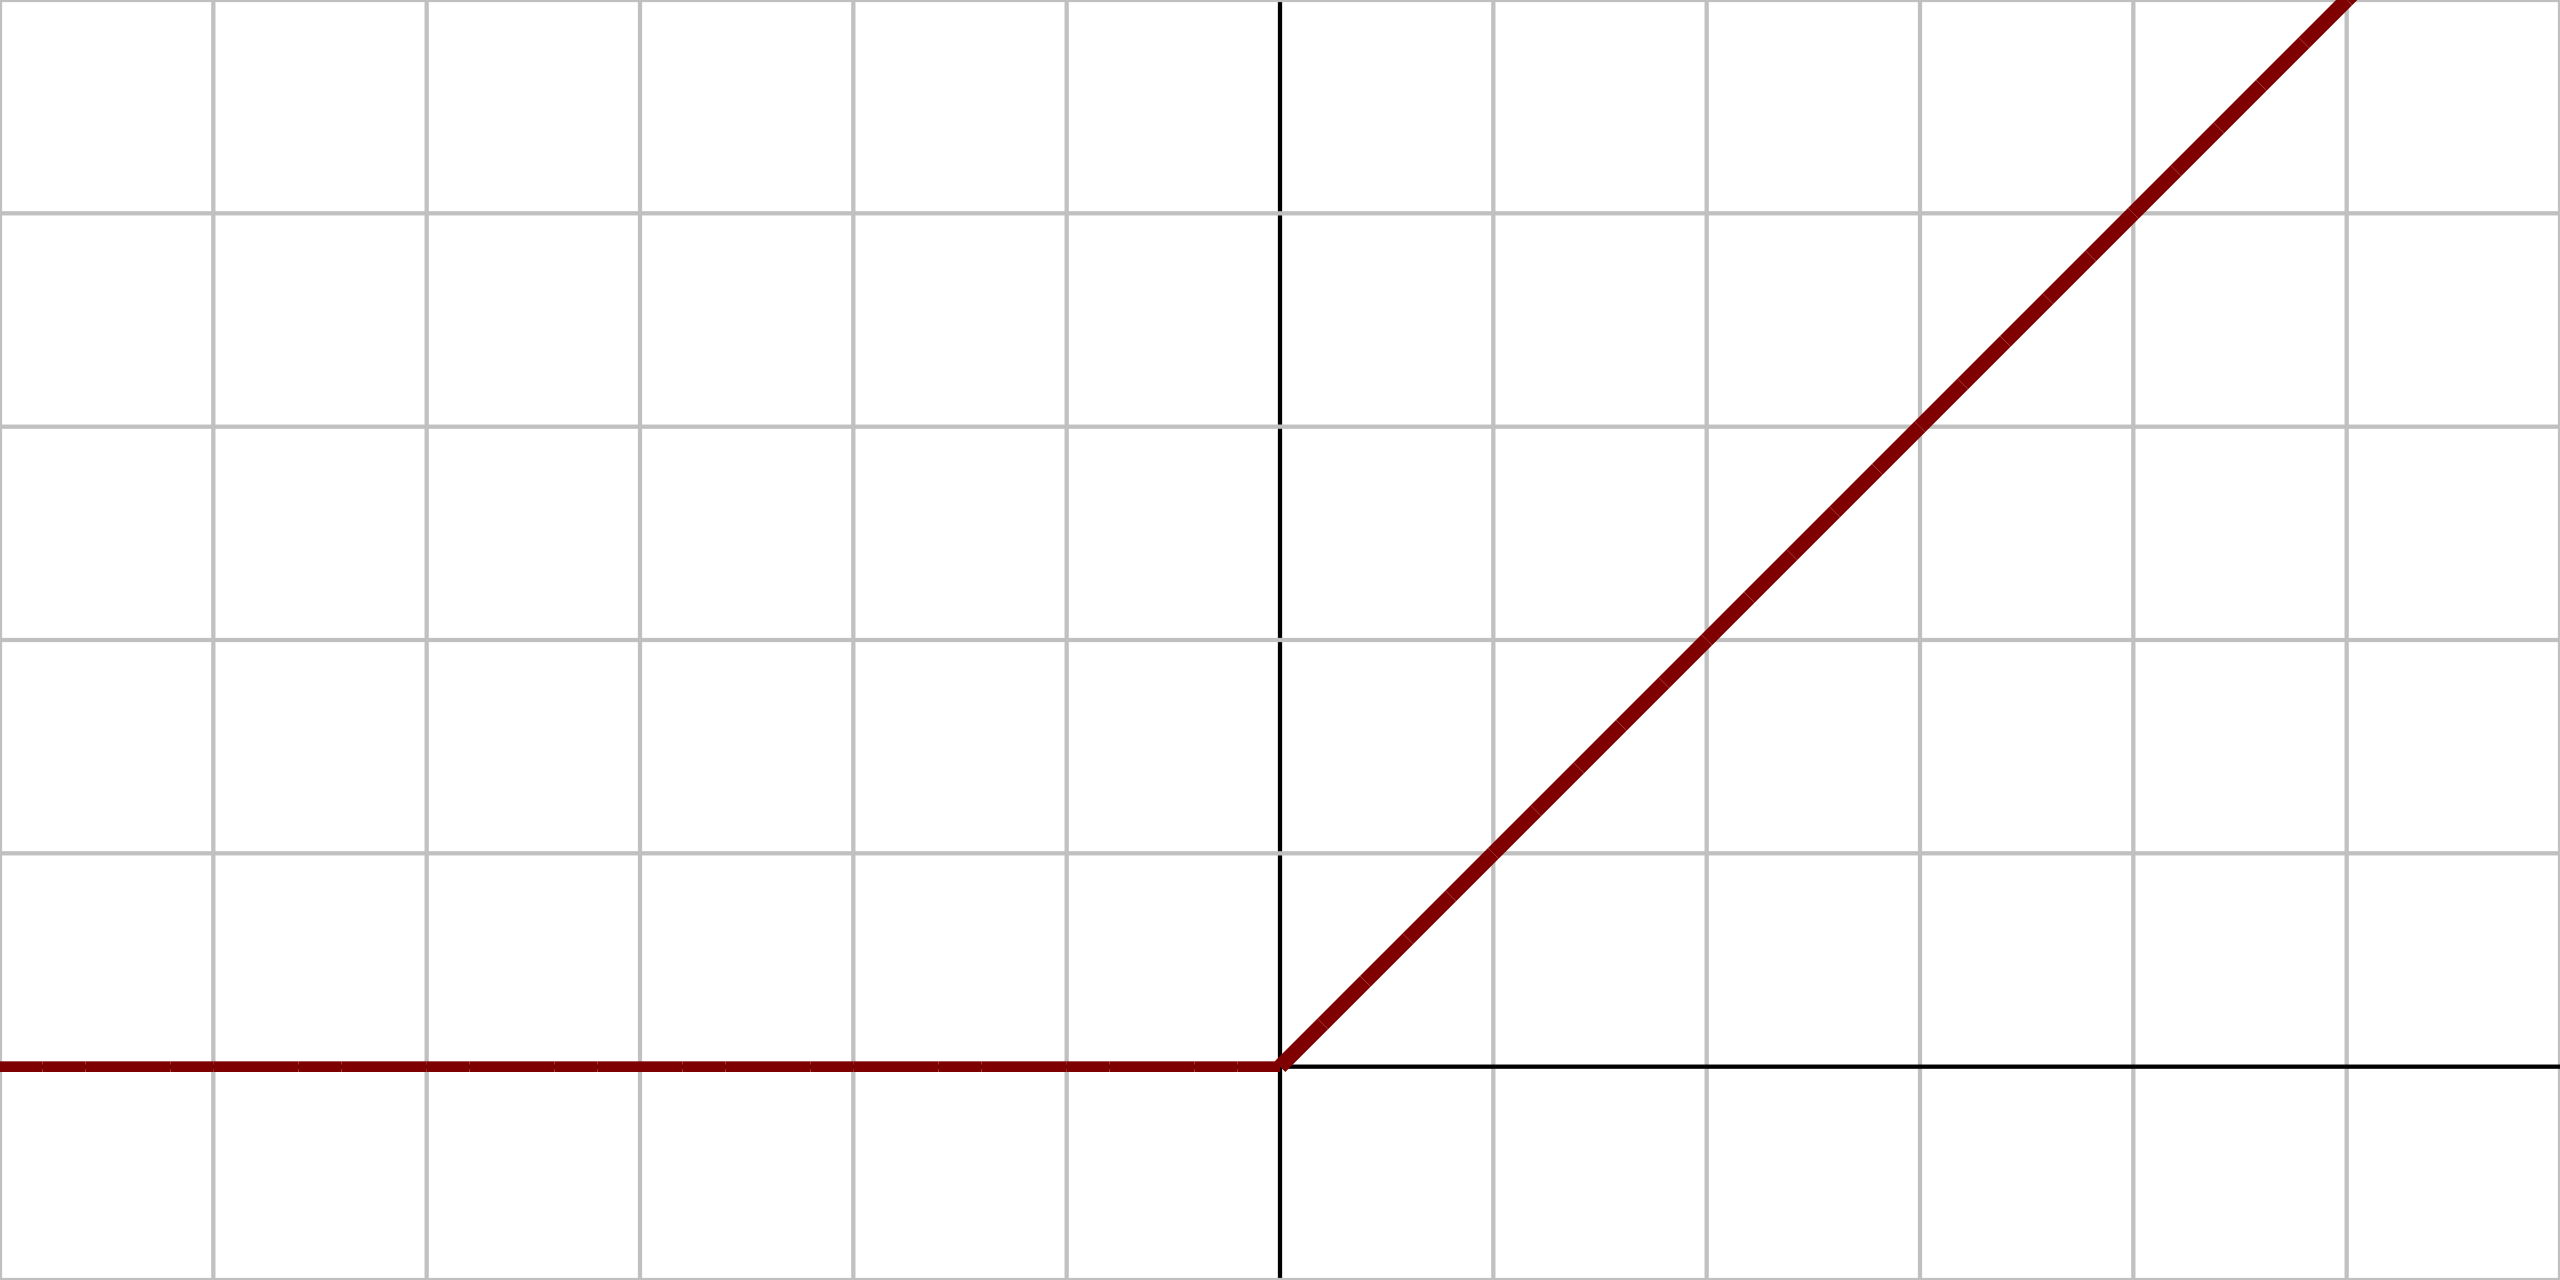
\includegraphics[width=1in]{relu.png} \\ \hline
%Leaky ReLU & $\displaystyle \begin{cases}
%0.01z & \text{if} z \leq 0 \\
%z & \text{if} z > 0
%\end{cases}$ & 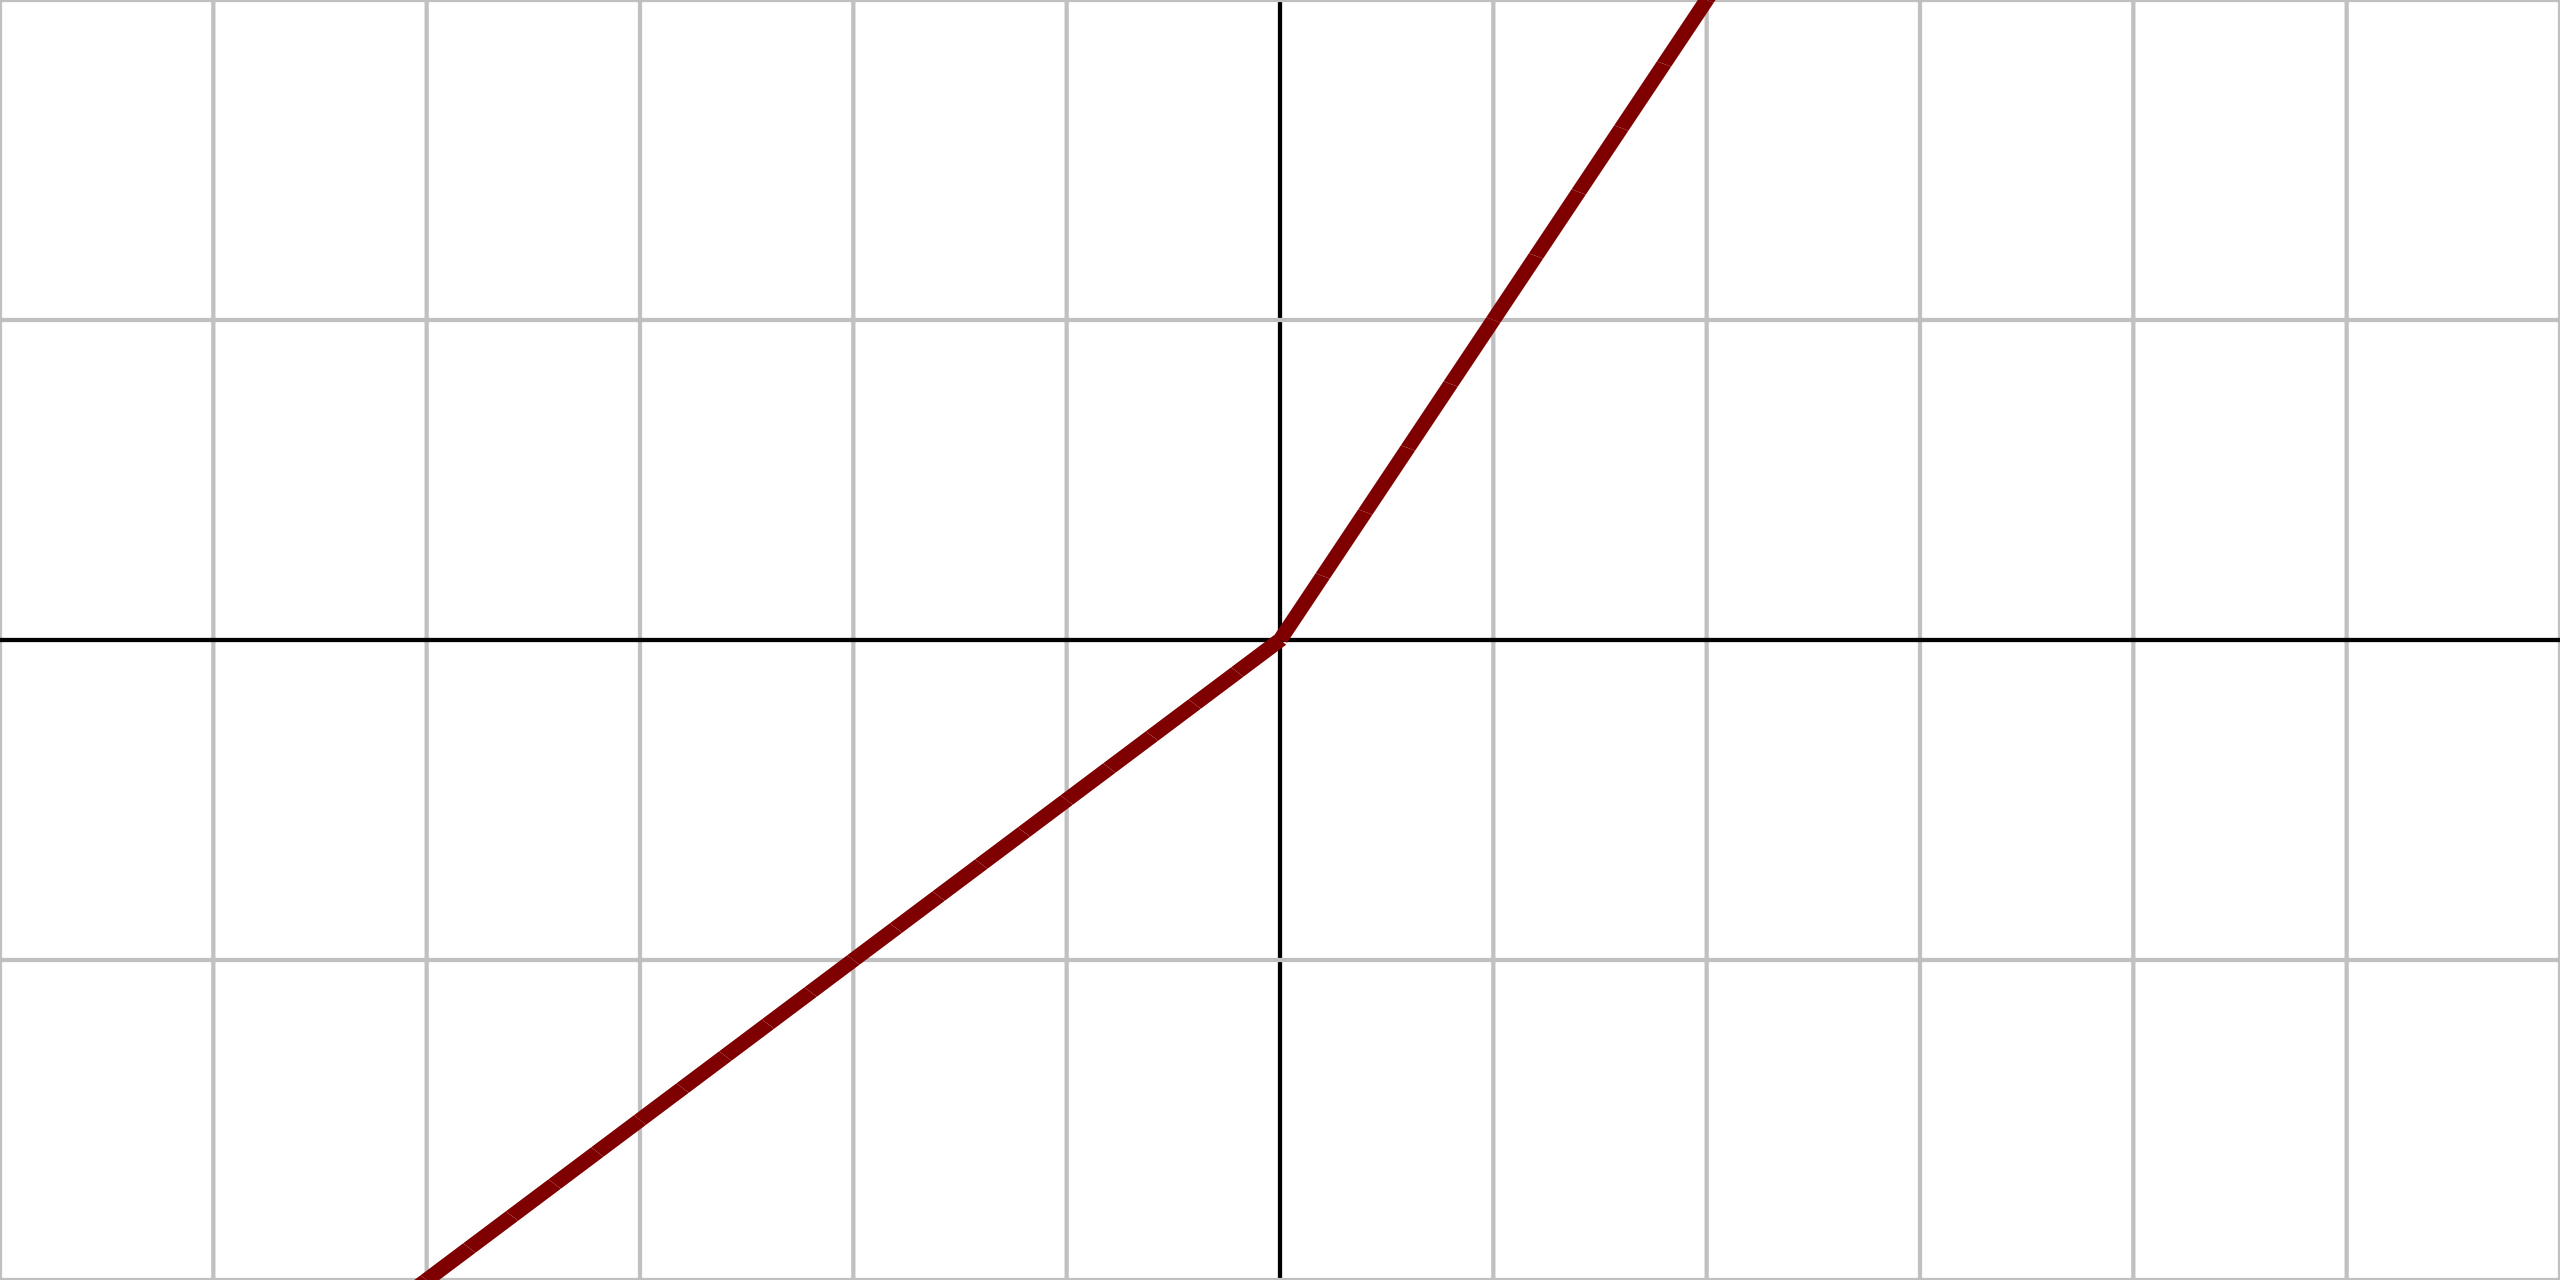
\includegraphics[width=1in]{leaky_relu.png} \\ \hline
%\end{tabular} \\

%\tiny Image sources:
%\url{https://commons.wikimedia.org/wiki/File:Activation_logistic.svg}, 
%\url{https://commons.wikimedia.org/wiki/File:Activation_rectified_linear.svg}, 
%\url{https://commons.wikimedia.org/wiki/File:Activation_gelu.png}, 
%\url{https://commons.wikimedia.org/wiki/File:Activation_tanh.svg}, 
%\url{https://commons.wikimedia.org/wiki/File:Activation_prelu.svg}
%\end{frame}

\begin{frame}{Popular Activation Functions}
\footnotesize
\renewcommand{\arraystretch}{1.5}

\begin{tabular}{l|l} 
Sigmoid & $\sigma(z) = \frac{e^z}{1+e^z}$  \\ \hline
Hyperbolic tangent & $\tanh(z)=\frac{sinh(z)}{cosh(z)} = \frac{e^z-e^{-z}}{e^z+e^{-z}} = 2\sigma(2z)-1$  \\ \hline
Softplus & $\sigma_+(z) = \log(1+e^a)$ \\ \hline
Rectified linear unit & $\operatorname{ReLU}(z) = \max(a, 0) $ \\ \hline
Leaky ReLU & $\operatorname{LReLU}(z)=\max(z, 0) + \alpha \min(z, 0)$  \\ \hline
Exponential linear unit & $\operatorname{ELU}(z) = \max(z, 0) + \min(\alpha(e^z-1), 0)$ \\ \hline
Swish, Sigmoid linear unit & $\operatorname{SiLU}(z) = z \sigma(z)$ \\ \hline
Gaussian error linear unit & $\operatorname{GeLU}(z) = z \Phi(z)$ \\ 
\end{tabular}
\vspace{\baselineskip}
\begin{columns}
\begin{column}{\textwidth}
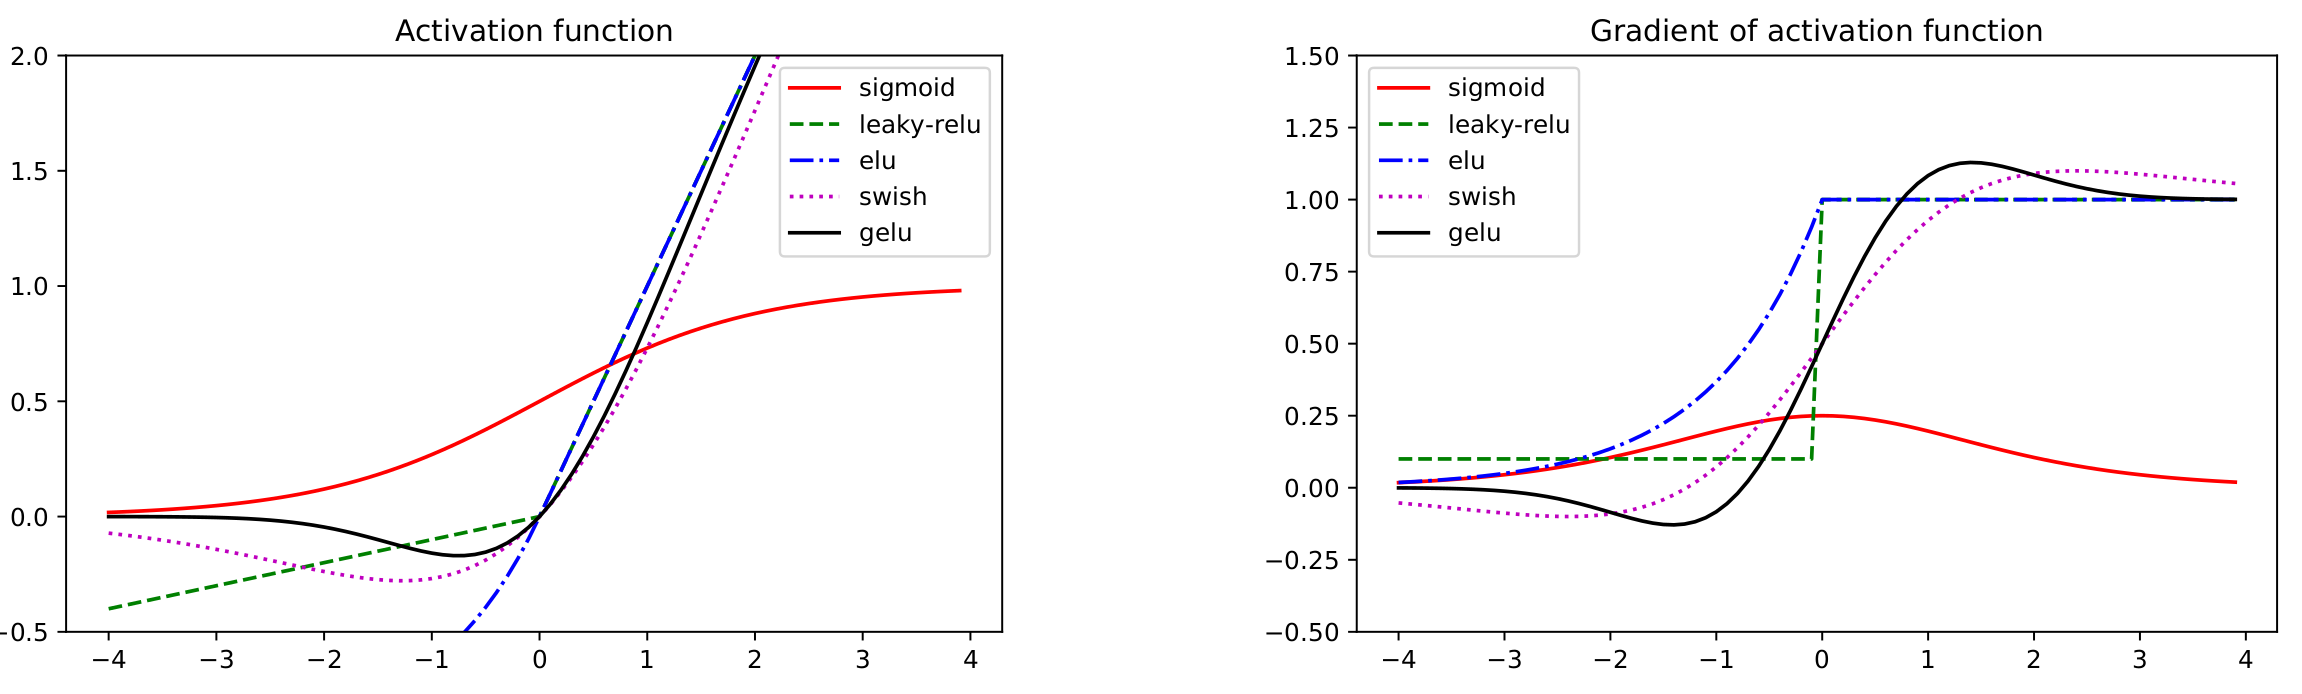
\includegraphics[width=\textwidth]{screen6}
\end{column}
\begin{column}{0.1\textwidth}
\scriptsize Source: Murphy, Fig. 13.14
\end{column}
\end{columns}
\end{frame}



\begin{frame}{Fully Connected Hidden Layer}
\centering
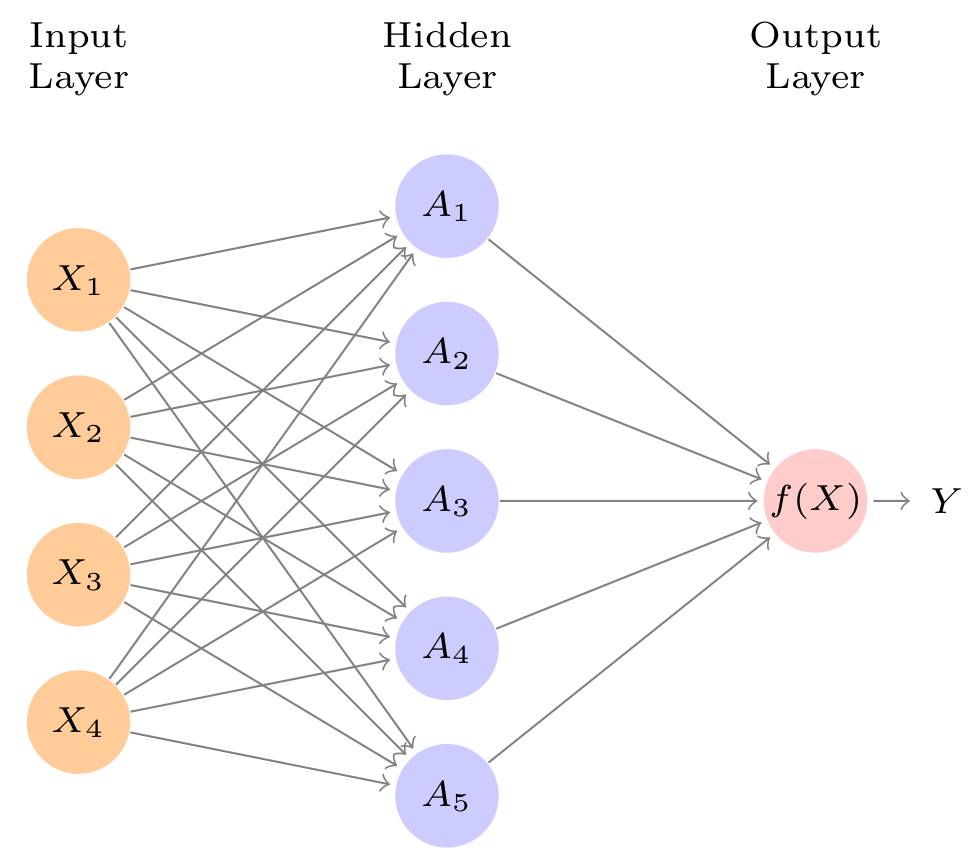
\includegraphics[height=2.75in]{screen1.png} \\

\scriptsize Source: ISLR2 Figure 10.1
\end{frame}

\begin{frame}{Fully Connected Multilayer Network}
\begin{columns}
\begin{column}{.66\textwidth}
\centering
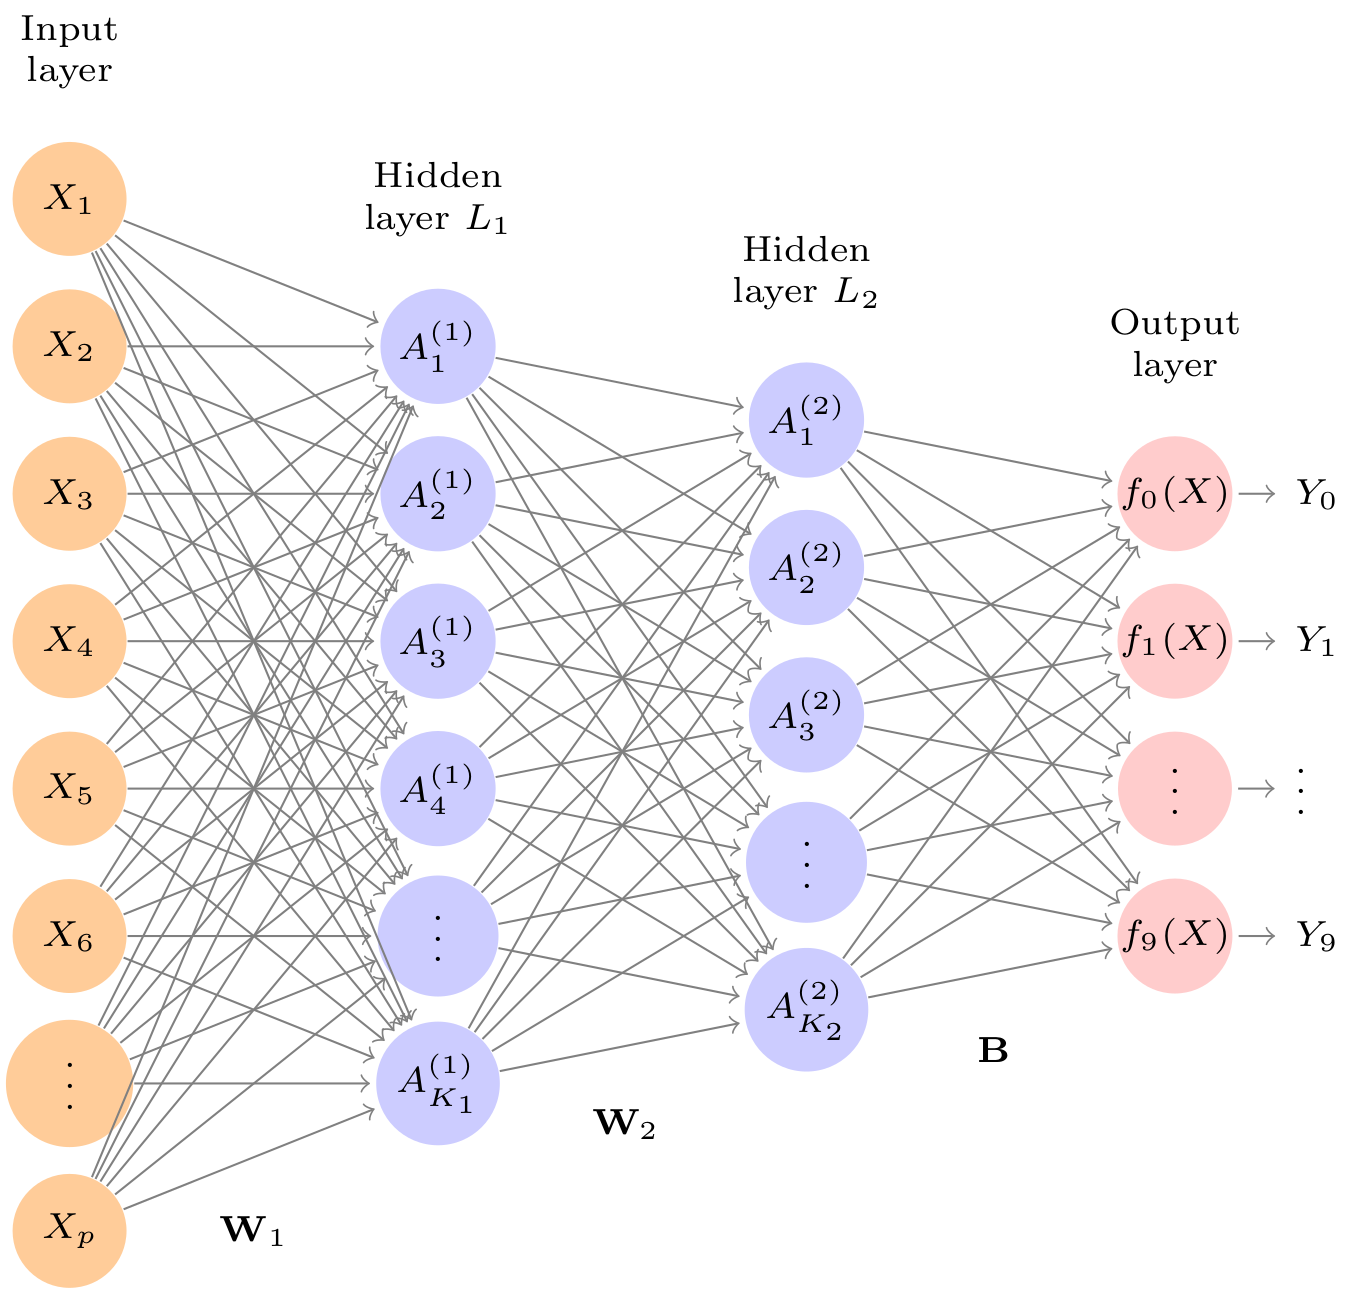
\includegraphics[width=\textwidth]{screen2.png} \\

\scriptsize Source: ISLR2 Figure 10.4
\end{column}
\begin{column}{.33\textwidth}
Multiple Outputs either
\begin{itemize}
   \item Multi-objective learning
   \item Multi-class classification
\end{itemize}
\vspace{\baselineskip}

''\textbf{Softmax}'' activation
\begin{align*}
\Pr(Y=m|X) = \frac{e^{Z_m}}{\sum_{l=0}^n e^{Z_l}}
\end{align*}
\end{column}
\end{columns}
\end{frame}

\begin{frame}{Estimating Parameters}
\footnotesize
\begin{block}{Typical Loss Functions}
\begin{itemize}  
  \item \textbf{Regression}: MSE, MAE, Huber
  \item \textbf{Classification}: Cross-Entropy or KL-Divergence after softmax on multiple output nodes 
\end{itemize}
\end{block}
\begin{block}{Parameters}
\begin{itemize}
  \item Parameter vector $\theta = (w, b)$ with weights $w$ and biases $b$. 
\end{itemize}
\end{block}
\begin{block}{Optimization}
\begin{itemize}
  \item (Stochastic) gradient descent (SGD)
\end{itemize}
\end{block}
\begin{block}{Regularization}
\begin{itemize}
  \item ''Dropout''
  \item L1 and/or L2 penalization (as in lasso, ridge)
  \item Early stopping
\end{itemize}
\end{block}
\end{frame}

\begin{frame}{Gradient Descent}
\begin{enumerate}
   \item Begin with initial parameter values
   \item Repeat until convergence
   \begin{enumerate}
      \item Find direction of descent (decrease in loss function value, given by the gradient vector $\nabla L$ of partial derivatives)
      \item Move a step in that direction (adjust parameters, step size determined by \textbf{learning rate})
   \end{enumerate}
\end{enumerate}
\begin{columns}
\begin{column}{0.6\textwidth}
\vspace{\baselineskip} 

Consider the loss $L$ at a certain input $X$ as a function of parameter values $\theta$. Then, at each step $t$, update parameters $\theta$ using learning rate $\gamma$:
\begin{align*}
\theta_{t+1} = \theta_t - \gamma \nabla L(\theta) \rvert_{\theta_t, X}
\end{align*}
\end{column}
\begin{column}{0.4\textwidth}
\centering
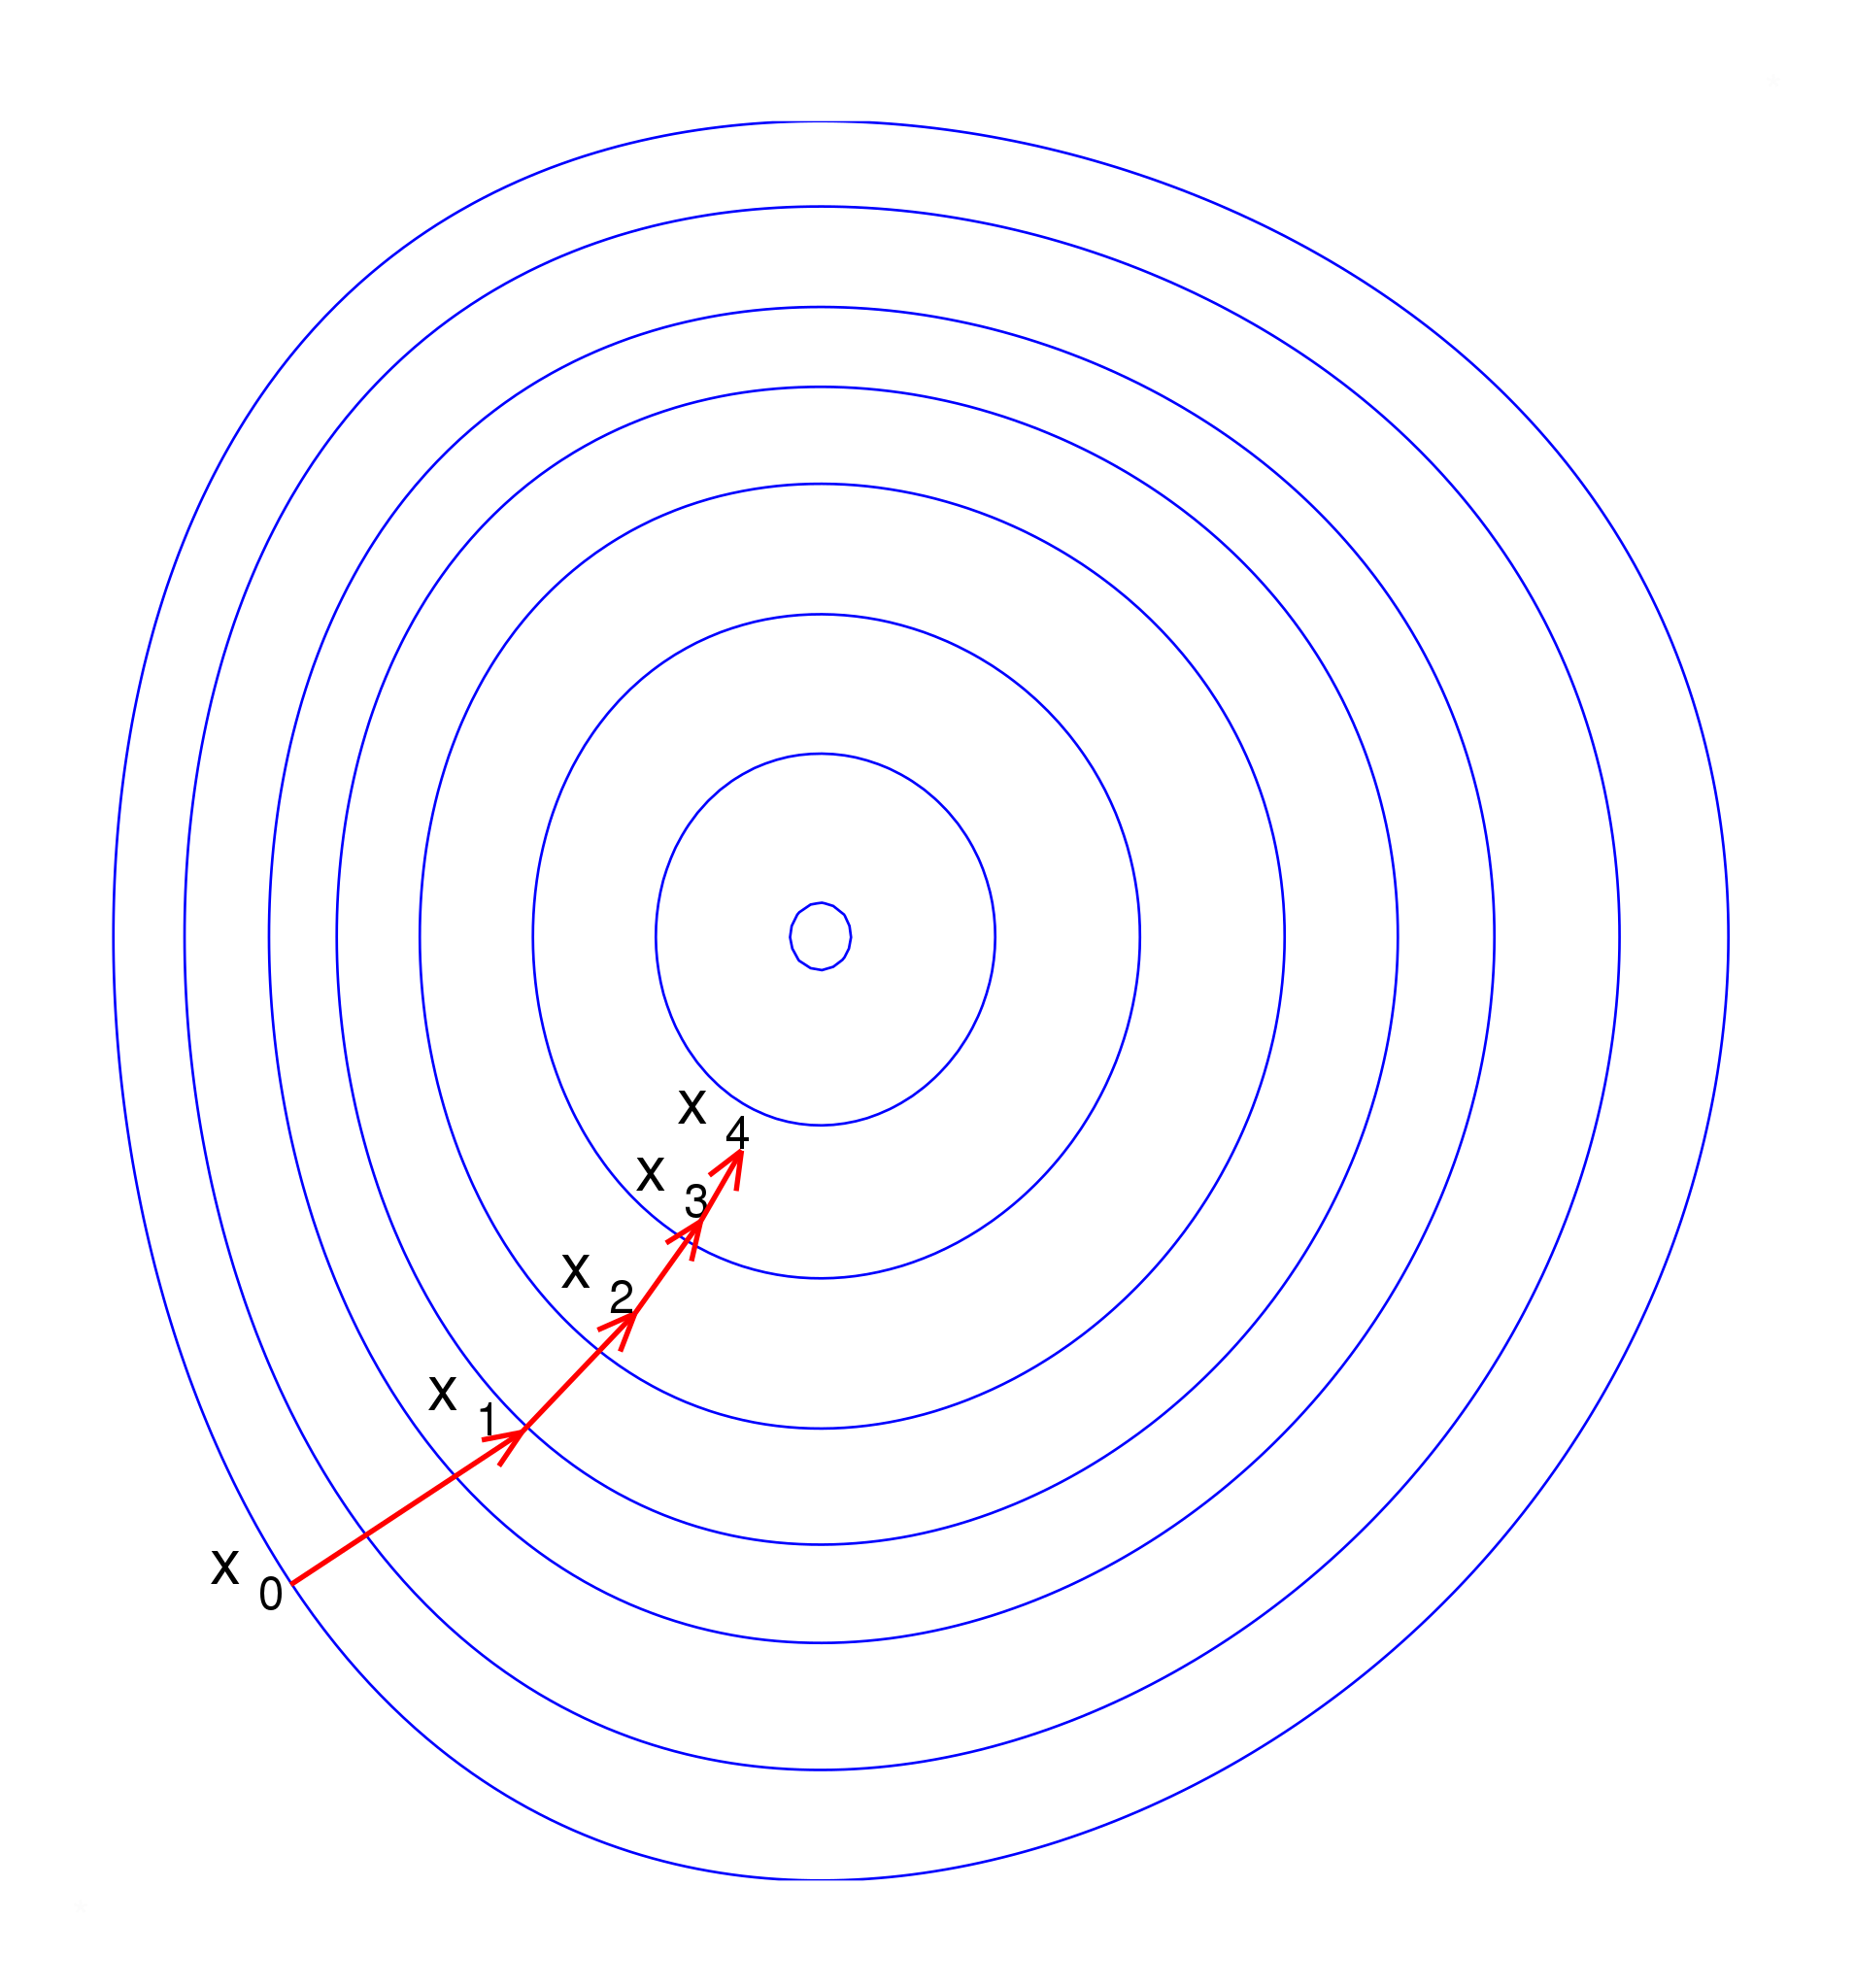
\includegraphics[width=\textwidth]{gradient_descent.png}
\end{column}
\end{columns}

\scriptsize \url{https://commons.wikimedia.org/wiki/File:Gradient_descent.svg}
\end{frame}

\begin{frame}{Optimization Problems}
\begin{itemize}
   \item Slow convergence
   \item No convergence (oscillations)
   \item Premature convergence (local optimimum)
\end{itemize}
\centering
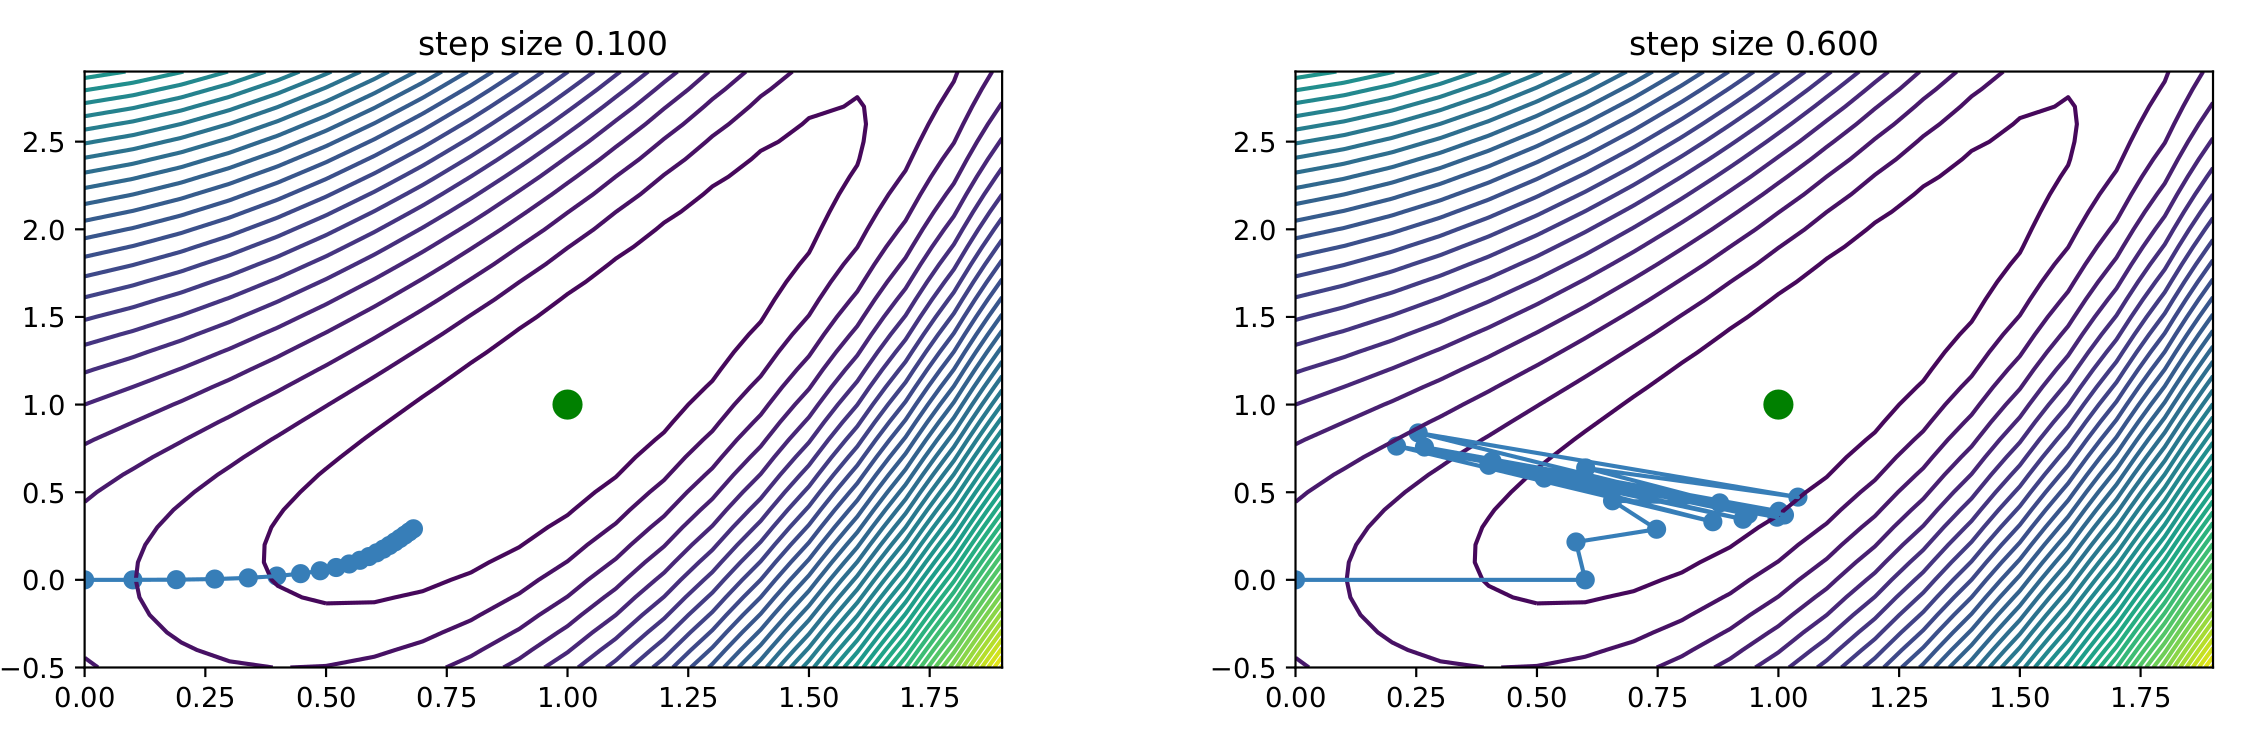
\includegraphics[width=\linewidth]{screen4} \\

\scriptsize Murphy, Figure 8.11
\end{frame}

\begin{frame}{Optimization Options}
\begin{block}{Learning Rate}
\begin{itemize}
   \item Fixed step size
   \item Adaptive learning rate $\lambda_t$
   \item Momentum methods
   \item Optimal learning rate (''line search'')
\end{itemize}
\end{block}
\end{frame}

\begin{frame}{Training Neural Networks -- Epochs and Minibatches}
\begin{itemize}
  \item Using the full training set for every update step is expensive (or impossible)
  \item Approximate true gradient by using a small sample of the training set for each step, the \textbf{minibatch}
  \begin{itemize}
     \item Average gradients over minibatch
     \item Minibatch should be independent and random
     \item Minibatch size should not be ''too small''
  \end{itemize}
  \item Multiple passes over the training set until convergence (a local or global optimimum is found), the \textbf{epochs}
  \begin{itemize}
     \item Avoid repetition by shuffling the training set before each epoch
     \item Early stopping for regularization
  \end{itemize}
\end{itemize}
\end{frame}


\begin{frame}{Optimization Options -- Stochastic Gradient Descent}
\begin{itemize}
   \item Random inputs $X$ to gradients by random draws from training set
\begin{align*}
\theta_{t+1} = \theta_t - \lambda_t \nabla L(\theta) \rvert_{\theta_t, X}
\end{align*}
\vspace{-\baselineskip}
   \item Requires adaptive learning rate
   \item Typical learning rate schedules: Piecewise constant, exponential decay, polynomial decay
\end{itemize}
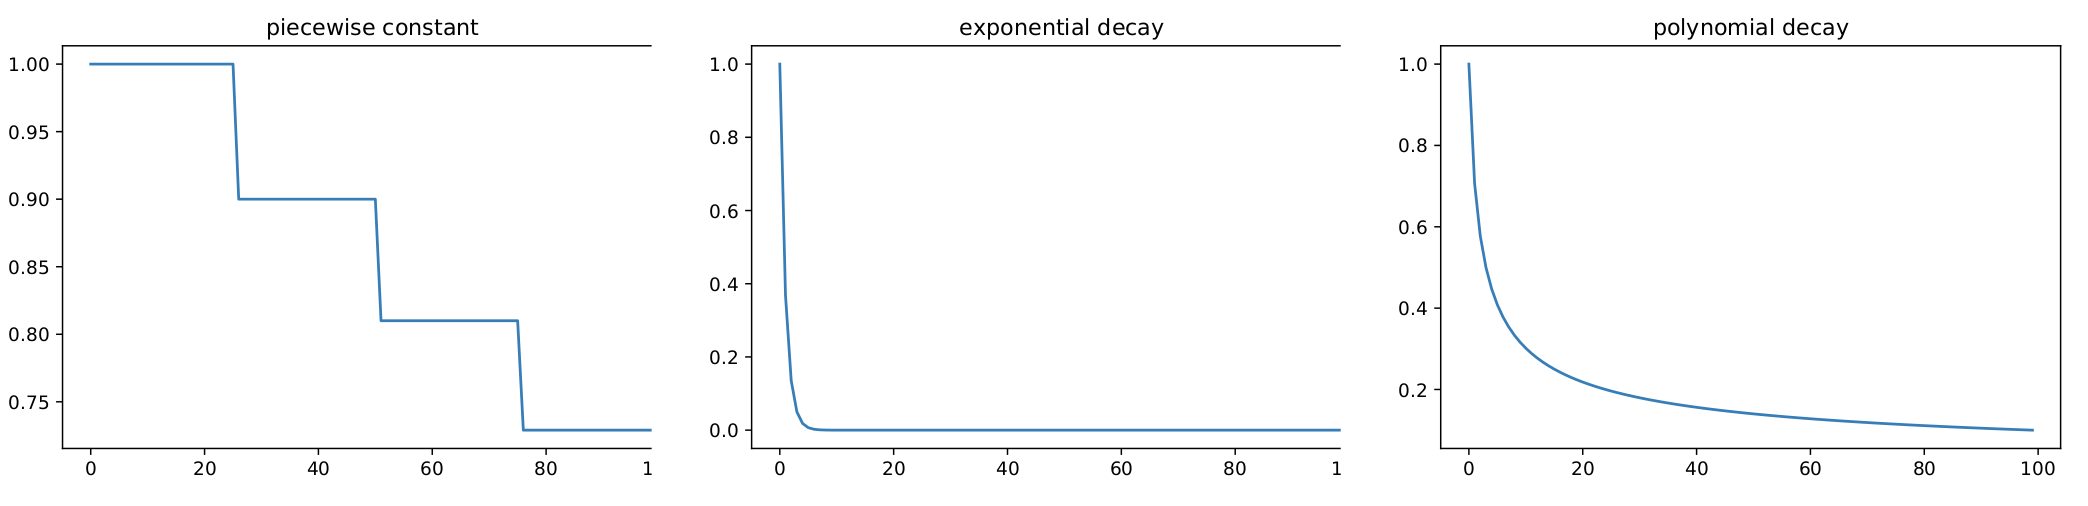
\includegraphics[width=\textwidth]{screen5.png} \\

\scriptsize Source: Murphy Figure 8.18
\end{frame}


\begin{frame}{Optimization Options -- AdaGrad}{Adaptive Gradient}
\begin{itemize}
  \item Originally developed for sparse gradient vectors
  \item Adapt by previous squared gradients
  \item Overall learning rate $\lambda_t$ is adapted
  \item Typically: $\lambda_t = \lambda_0$
\end{itemize}
\begin{align*}
\theta_{t+1} &= \theta_t - \lambda_t \frac{1}{\sqrt{s_t + \epsilon}}\nabla L(\theta) \rvert_{\theta_t, X} \\
s_t &= \sum_{\tau=1}^t \left( \nabla L(\theta)\rvert_{\theta_\tau, X}\right)^2 \quad \text{Sum of squared gradients}
\end{align*}
\end{frame}

\begin{frame}{Optimization Options -- RMSProp}
\begin{itemize}
   \item Exponentially weighted moving average of the past (instead of the sum as in AdaGrad)
   \item Prevents too early learning rate reduction
\end{itemize}
\begin{align*}
s_{t+1} &= \beta s_t + (1-\beta) \left( \nabla L(\theta)\rvert_{\theta_t, X}\right)^2 
\end{align*}
\end{frame}

\begin{frame}{Optimization Options -- AdaDelta}
\begin{itemize}
  \item Maintains exponentially weighted average of previous updates $\delta$
\end{itemize}
\begin{align*}
\theta_{t+1} &= \theta_t + \Delta\theta_t \\
\Delta\theta_{t} &= - \lambda_t \frac{\sqrt{\delta_{t-1} + \epsilon}}{\sqrt{s_t + \epsilon}} \nabla L(\theta) \rvert_{\theta_t, X} \\
\delta_t &= \beta \delta_{t-1} + (1-\beta) (\Delta\theta_t)^2
\end{align*}
\end{frame}

\begin{frame}{Optimization Options -- Momentum Methods}
\begin{itemize}
  \item \emph{Intuition}: Keep going in the direction that was previously good, avoid ''sharp turns''
  \item Standard momentum:
\begin{align*}
m_{t+1} &= \beta m_{t} - \nabla L(\theta) \rvert_{\theta_t, X} &\qquad \text{Momentum} \\
\theta_{t+1} &= \theta_{t} - \lambda m_{t+1} &\qquad \text{Parameter update} \\
& &\text{Typical $\beta$ is} \approx 0.9
\end{align*}
  \item Nesterov Momentum: Looks ahead and evaluates gradient at approximate next parameter values
\begin{align*}
m_{t+1} &= \beta m_{t} - \lambda_t \nabla L(\theta) \rvert_{\theta_{t}+\beta m_{t}, X} &\qquad \text{Nesterov Momentum} \\
\theta_{t+1} &= \theta_{t} + m_{t+1} &\qquad \text{Parameter update}
\end{align*}
\end{itemize}
\end{frame}


\begin{frame}{Optimization Options -- AdaM}{Adaptive Moment Estimation}
\begin{itemize}
  \item Combine adaptive learning rate with momentum
\end{itemize}
\begin{align*}
m_t &= \beta_1 m_{t-1} + (1-\beta_1) \nabla L(\theta)\rvert_{\theta_t, X} \\
s_t &= \beta_2 s_{t-1} + (1-\beta_2) \left( \nabla L(\theta)\vert_{\theta_t, x} \right)^2 \\
\theta_{t+1} &= \theta_t - \lambda_t \frac{1}{\sqrt{s_t}+\epsilon} m_t 
\end{align*}
\end{frame}


\begin{frame}{Training Neural Networks -- Vanishing Gradients }
\begin{block}{Problem}
\begin{itemize}
  \item Sigmoid and tanh functions are bounded for large positive or negative pre-activation values (''saturating activation functions'')
  \item Long chains of neurons (e.g. in stacked fully-connected layers) can diminish the ''error signal'', i.e. the gradient
\end{itemize}
\end{block}
\begin{block}{Possible Solutions}
\begin{itemize}
  \item Use non-saturating activation functions, e.g. ReLU, leaky ReLU, ELU, etc.
  \item Use additive rather multiplicative architectures, e.g. ''ResNet'' (residual networks)
  \item Standardize activations at every layer
  \item Carefully choose initial parameter values
\end{itemize}
\end{block}
\end{frame}


\begin{frame}{Training Neural Networks -- ResNet Architecture}
\begin{itemize}
  \item Allows gradients to bypass a layer that suffers from lack of learning (vanishing gradient, saturated activation)
\end{itemize}
\centering
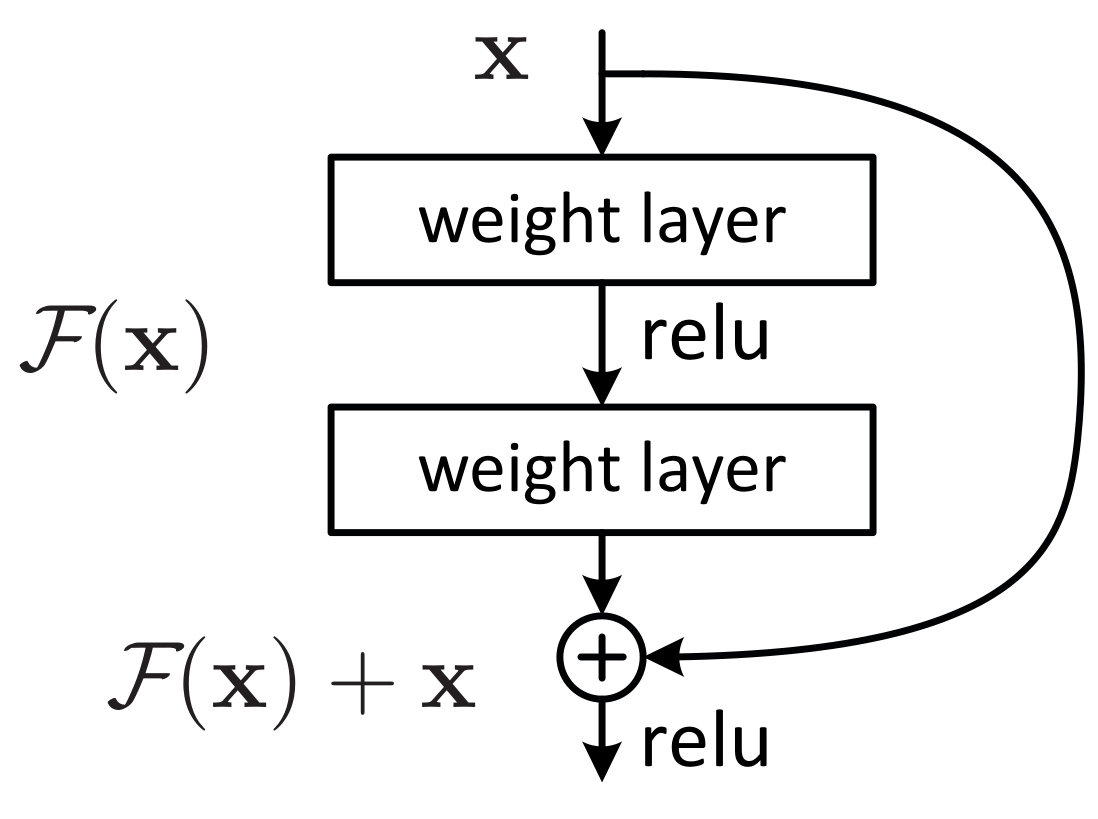
\includegraphics[height=2in]{screen8.png} \\

\scriptsize Source: Murphy, Figure 13.15
\end{frame}


\begin{frame}{Training Neural Networks -- Exploding Gradients }
\begin{block}{Problem}
\begin{itemize}
   \item Long chains of neurons can vastly increase the error
\end{itemize}
\end{block}
\begin{block}{Possible Solution}
\begin{itemize}
   \item Gradient clipping
\begin{align*}
g' = min(1, \frac{1}{||c||_2}) g
\end{align*}
\end{itemize}
\end{block}
\end{frame}

\begin{frame}{Training Neural Networks -- Parameter Initialization Heuristics}
\begin{itemize}
  \item Random values from normal distribution: $\theta \sim N(0, \sigma^2)$
  \item ''Xavier Initialization''/''Glorot Initialization''
\begin{align*}
  \sigma^2 = \frac{2}{n_{\text{in}} + n_{\text{out}}}
\end{align*}
   where $n_{\text{in}}$ is the number of incoming connections and $n_{\text{out}}$ is the number of outgoing connections from each neuron
   \item ''LeCun Initialization''
\begin{align*}
  \sigma^2 = \frac{1}{n_{\text{in}}}
\end{align*}
   \item ''He Initialization''
\begin{align*}
  \sigma^2 = \frac{2}{n_{\text{in}}}
\end{align*}
\end{itemize}
\end{frame}


\begin{frame}{Regularization -- Dropout}
\begin{itemize}
   \item Randomly (per observation) remove a fraction of units in a layer, or equivalently,
   \item Randomly set the output of a fraction of units to 0
   \item Typically only done at train time, not test time
\end{itemize}
\centering
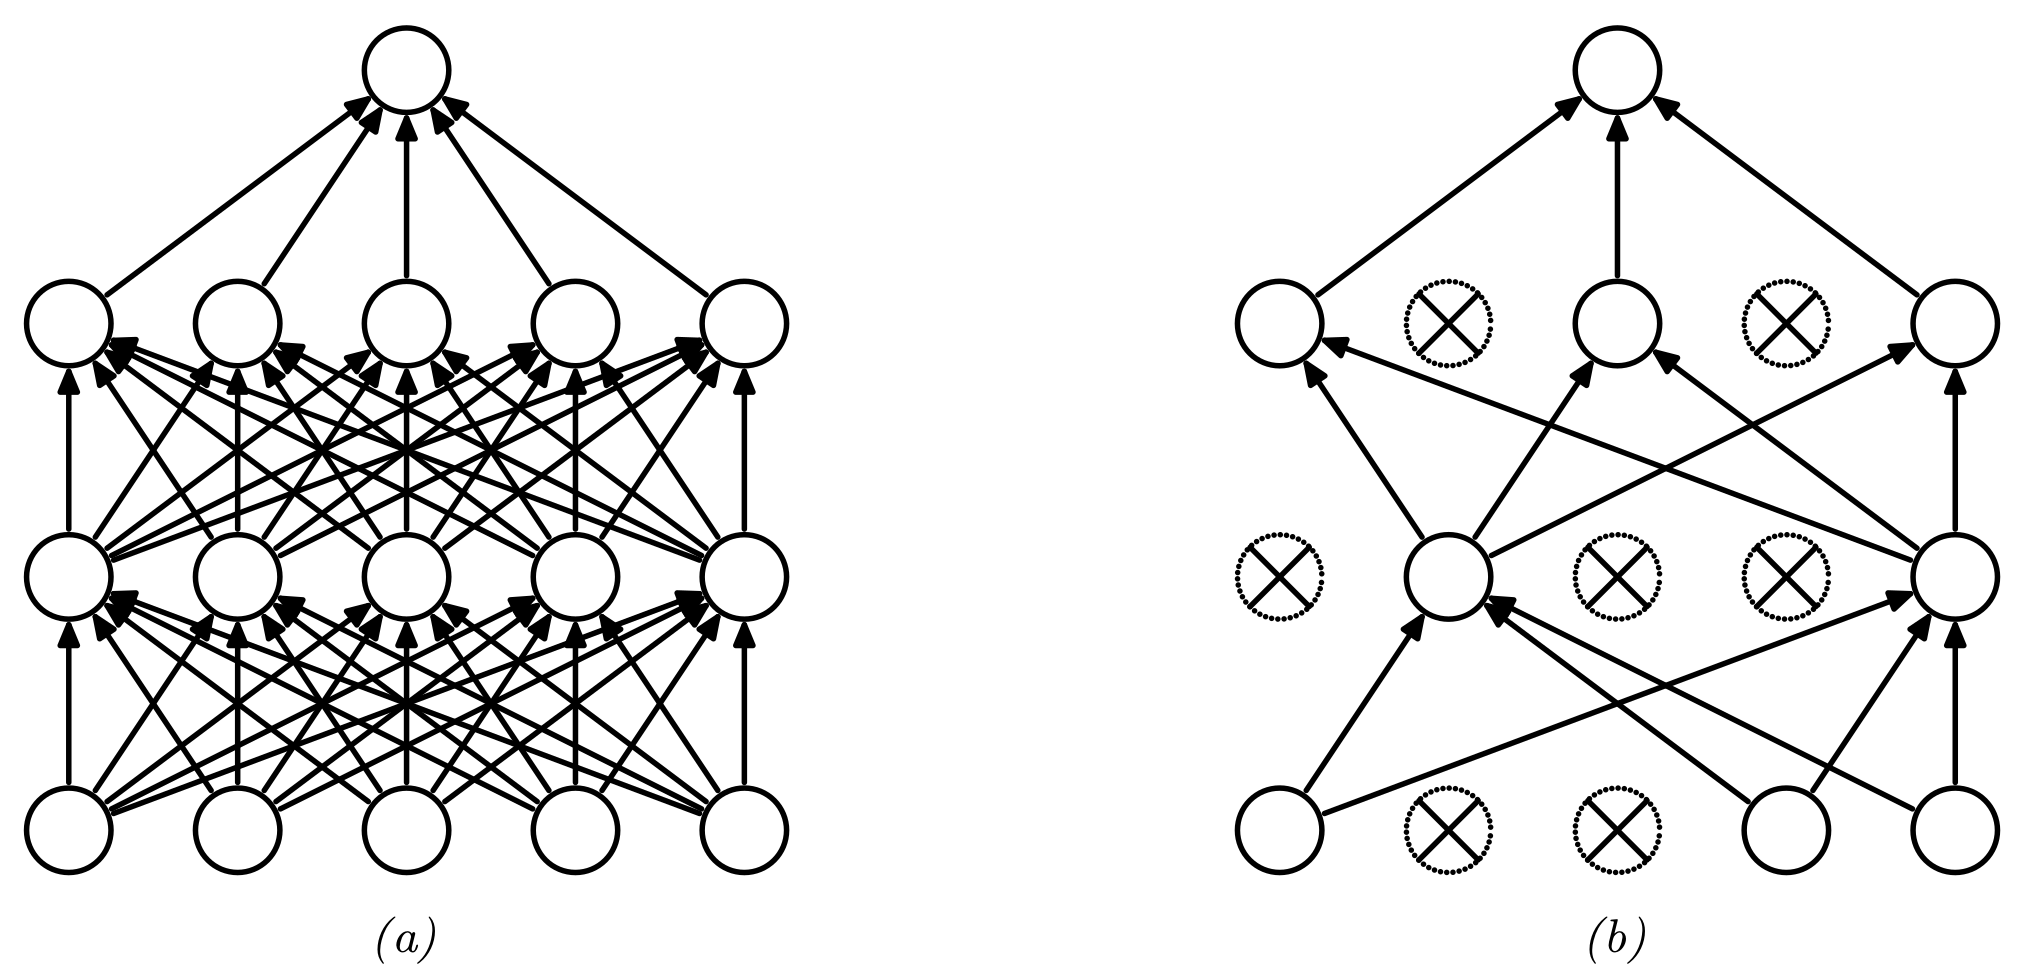
\includegraphics[height=1.8in]{screen7.png} \\

\scriptsize Source: Murphy, Figure 1.318
\end{frame}

\begin{frame}{Tensorflow}
\begin{columns}
\begin{column}{0.3\textwidth}

\includegraphics[width=\textwidth]{tflogo.png}
\end{column}
\begin{column}{0.7\textwidth}
\begin{itemize}
  \item Originally developed by Google, Version 1.0 in 2017
  \item Automatic differentiation/gradients
  \item Distributed computing
  \item Parallel computing on multiple GPU
  \item Wide range of loss functions
  \item Wide range of optimizers
  \item Wide range of neural network types and activation functions
\end{itemize}
\end{column}
\end{columns}
\end{frame}

\begin{frame}{Keras}
\begin{columns}
\begin{column}{0.3\textwidth}

\includegraphics[width=.75\textwidth]{keraslogo.png}
\end{column}
\begin{column}{0.7\textwidth}
\begin{itemize}
   \item Originally developed as a user-friendly, high-level abstraction layer for different ML frameworks, including Tensorflow, Theano, PyTorch
   \item Wide range of standard neural network layers
   \item Simplified training loops
\end{itemize}
\end{column}
\end{columns}
\end{frame}


\begin{frame}[fragile]{Regression using Keras}
Import required packages:
\begin{pythoncode}
import pandas as pd
import numpy as np
import tensorflow as tf
from tensorflow.keras import layers
\end{pythoncode}
Read a CSV file:
\begin{pythoncode}
# Use the Boston housing data set
boston_data = \
    pd.read_csv("https://evermann.ca/busi4720/boston.csv")
\end{pythoncode}
Separate features and target:
\begin{pythoncode}
boston_features = boston_data.copy()
boston_labels = boston_features.pop('medv')
\end{pythoncode}
\end{frame}


\begin{frame}[fragile]{Regression using Keras \small [cont'd]}
Define the NN model with one hidden fully-connected layer (64 neurons) and one fully-connected output layer (1 neuron) in sequence. No activation function is given, so this is a linear regression model:
\begin{pythoncode}
boston_model = tf.keras.Sequential([
  layers.Dense(64, activation=None),
  layers.Dense(1, activation=None)
])
\end{pythoncode}
Set the loss function and the optimizer:
\begin{pythoncode}
boston_model.compile(
    loss = tf.keras.losses.MeanSquaredError(),
    optimizer = tf.keras.optimizers.Adam())
\end{pythoncode}
Fit/train the model for 25 epochs:
\begin{pythoncode}
boston_model.fit(boston_features, 
                 boston_labels, epochs=25)
boston_model.summary()
\end{pythoncode}
\end{frame}

\begin{frame}[fragile]{Regression in Keras \small [cont'd]}
The \texttt{Normalization} layer normalizes numeric features:
\begin{pythoncode}
norm_layer = layers.Normalization()
\end{pythoncode}
The \texttt{adapt()} function computes means and variances of the data so the layer can normalize the data when the model is fit. Requires numpy array.
\begin{pythoncode}
norm_layer.adapt(boston_features.to_numpy())
\end{pythoncode}
Add the normalization layer to the model. A ReLU activation is used that makes this a non-linear regression model:
\begin{pythoncode}
norm_boston_model = tf.keras.Sequential([
  norm_layer,
  layers.Dense(64, activation='relu'),
  layers.Dense(1, activation=None)
])
\end{pythoncode}
\end{frame}

\begin{frame}[fragile]{Regression in Keras \small [cont'd]}
Set loss and optimizer and ask Keras to keep track of the MSE and MAE metrics.
\begin{pythoncode}
norm_boston_model.compile(
    loss = tf.keras.losses.MeanSquaredError(),
    optimizer = tf.keras.optimizers.Adam(),
    metrics = ['mse', 'mae'])
\end{pythoncode}
The \texttt{fit} function returns a history of the metrics we asked for:
\begin{pythoncode}    
train_hist = \
    norm_boston_model.fit(
        boston_features, 
        boston_labels, 
        batch_size=20,
        epochs=50,
        validation_split=0.33)
\end{pythoncode}
\end{frame}

\begin{frame}[fragile]{Regression in Keras \small [cont'd]}
Plot the training history using Plotly Express
\begin{pythoncode}
import plotly.express as px

hist = pd.DataFrame({
    'training': train_hist.history['mse'],
    'validation': train_hist.history['val_mse']})
hist['epoch'] = np.arange(hist.shape[0])
hist = pd.melt(hist, 
               id_vars='epoch', 
               value_vars=['training', 'validation'])

fig = px.line(hist, x='epoch', y='value', 
                    color='variable')
fig.show()
\end{pythoncode}
\end{frame}

\begin{frame}{Hands-On Exercises}
\begin{itemize}
  \item Modify the above code to include different activation functions, e.g. \texttt{"tanh"}, \texttt{"sigmoid"}, or \texttt{"elu"}. Comment on the learning progress and loss function values.
  \item Modify the above code to change the number of neurons in the \texttt{"Dense"} layer. Comment on the learning progress and loss function values.
  \item Modify the architecture to add one or more \texttt{"Dense"} layers with different numbers of units. Comment on the learning progress and loss function values.
\end{itemize}
\end{frame}


\begin{frame}[fragile]{Classification in Keras}

The \texttt{Wage} dataset from the ISLR2 library for R has been adapted to include a column \texttt{wagequart}, the quartile of the wage. Many features are categorical.

\begin{pythoncode}
# Read data and separate features from target labels
wage_data = \
    pd.read_csv("https://evermann.ca/wage.csv")
    
wage_features = wage_data.copy()
wage_labels = wage_features.pop('wagequart') - 1
\end{pythoncode}
\end{frame}

\begin{frame}[fragile]{Classification in Keras \small [cont'd]}

Treat each categorical string feature and convert to \textbf{one-hot encoding}. \\

One-hot encoding is similar to binary dummy variables (contrasts) in linear models, but have no default level; a feature with $n$ different categories requires $n$ binary variables (not $n-1$ as in linear model contrasts). \\

Keep track of the inputs and the pre-processed inputs:
\begin{pythoncode}
inputs = {}
preproc_inputs = []
\end{pythoncode}
\end{frame}

\begin{frame}[fragile]{Classification in Keras \small [cont'd]}
\begin{pythoncode}
for cat_feature in ['maritl', 'race', 'education', \
               'jobclass', 'health', 'health_ins']:
    # An Input variable is a placeholder that
    # accepts data input when training or predicting
    input = tf.keras.Input(shape=(1,), 
                           name=cat_feature, 
                           dtype=tf.string)
    # This StringLookup layer accepts a string and 
    # outputs its category as a one-hot vector
    lookup = layers.StringLookup(
        name=cat_feature+"_lookup",
        output_mode="one_hot")
    # Adapt it to the different strings in the data
    lookup.adapt(wage_features[cat_feature])
    # And tie the input to this layer
    onehot = lookup(input)
    
    inputs[cat_feature] = input
    preproc_inputs.append(onehot)
\end{pythoncode}
\end{frame}

\begin{frame}[fragile]{Classification in Keras \small [cont'd]}
Define and input and a \texttt{Normalizaton} layer for the numerical variable \texttt{age}:
\begin{pythoncode}
age_input = tf.keras.Input(shape=(1,), 
                           name="age", 
                           dtype="float32")
norm_layer = layers.Normalization(name="age_norm")
norm_layer.adapt(wage_features["age"])
age_norm = norm_layer(age_input)

inputs["age"] = age_input
preproc_inputs.append(age_norm)
\end{pythoncode}
\end{frame}

\begin{frame}[fragile]{Classification in Keras \small [cont'd]}
Define and input and a one-hot encoding \texttt{IntegerLookup} layer for the numeric variable \texttt{year}:
\begin{pythoncode}
year_input = tf.keras.Input(shape=(1,), 
                           name="year", 
                           dtype="int32")
lookup = layers.IntegerLookup(name="year_lookup",
                              output_mode="one_hot")
lookup.adapt(wage_features["year"])
year_onehot = lookup(year_input)

inputs["year"] = year_input
preproc_inputs.append(year_onehot)
\end{pythoncode}
\end{frame}

\begin{frame}[fragile]{Classification in Keras \small [cont'd]}
Concatenate the pre-processing outputs to one long vector with a \texttt{Concatenate} layer. Call this layer with the list of prec-processed inputs:
\begin{pythoncode}
preprocessed_inputs = \
    layers.Concatenate(name="concat")(preproc_inputs)
\end{pythoncode}
Build a pre-processing model whose inputs is the dict of \texttt{Input} variables, and whose output are the results of calling the layers:
\begin{pythoncode}
preproc_model = tf.keras.Model(inputs, 
                               preprocessed_inputs,
                               name="preproc")
preproc_model.summary()
\end{pythoncode}
\end{frame}

\begin{frame}[fragile]{Classification in Keras \small [cont'd]}
Build the classification model as a \texttt{Sequential} model:
\begin{pythoncode}
class_model = tf.keras.Sequential(name="classification")
class_model.add(layers.Dense(64, activation="relu"))
class_model.add(layers.Dropout(0.25))
class_model.add(layers.Dense(32, activation="relu"))
class_model.add(layers.Dropout(0.25))
class_model.add(layers.Dense(4, activation="softmax"))

# Alternatively:
# class_model.add(layers.Dense(4, activation=None))
# class_model.add(layers.Softmax())
\end{pythoncode}
\end{frame}

\begin{frame}[fragile]{Classification in Keras \small [cont'd]}
The output of the pre-processing model is the input to the classification model:
\begin{pythoncode}
class_results = class_model(preproc_model(inputs))
class_model.summary()
\end{pythoncode}
The final model takes the inputs, and has the classification model results as outputs:
\begin{pythoncode}
wage_model = tf.keras.Model(inputs, class_results,
                            name="wage_model")
wage_model.summary()
\end{pythoncode}
\end{frame}

\begin{frame}[fragile]{Classification in Keras \small [cont'd]}
Compile the model with loss function, optimizer and request training metrics:
\begin{pythoncode}
wage_model.compile(
    loss=tf.keras.losses.SparseCategoricalCrossentropy(
       from_logits=False),
    optimizer=tf.keras.optimizers.Adam(
        learning_rate=0.001,
        beta_1 = 0.9,
        beta_2 = 0.999,
        epsilon = 1e-07),
    metrics=[
        tf.keras.metrics.SparseCategoricalAccuracy(), 
        tf.keras.metrics.KLDivergence()])
\end{pythoncode}
Note: Specifying \texttt{from\_logits=True} for the loss can save the softmax activation or layer at the bottom of the sequential classification model.
\end{frame}

\begin{frame}[fragile]{Classification in Keras \small [cont'd]}
Create the input data as a dict of numpy arrays to match the \texttt{Input} variables:
\begin{pythoncode}
import numpy as np
wage_feature_dict = \
    {name: np.array(value) for \
        name, value in wage_features.items()}
\end{pythoncode}
Write log information to a directory for loading into \textbf{Tensorboard}:
\begin{pythoncode}
import datetime
log_dir = "./tensorboard_logs/" + \
    datetime.datetime.now().strftime("%Y%m%d-%H%M%S")
tensorboard_callback = \
    tf.keras.callbacks.TensorBoard(log_dir=log_dir, 
        histogram_freq=0)
\end{pythoncode}
\end{frame}

\begin{frame}{TensorBoard}
TensorBoard is a tool to visualize neural network models and their trainging and validation data/performance.

\vspace{\baselineskip}
\centering
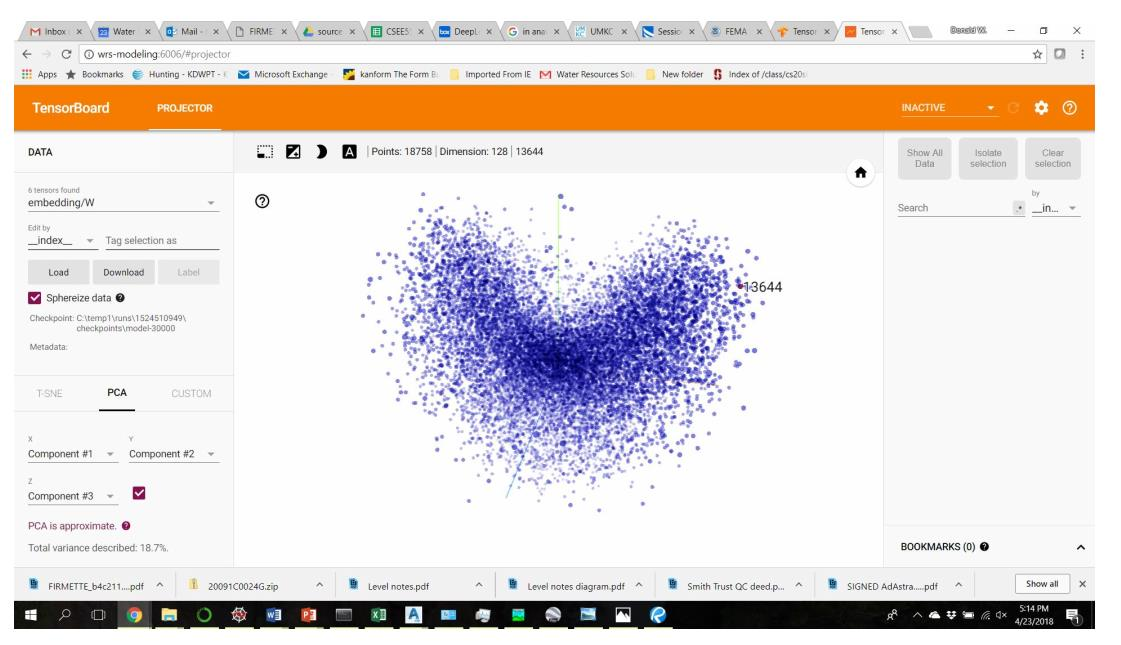
\includegraphics[width=.8\textwidth]{Tensorboard_1.jpg} \\

\scriptsize \url{https://commons.wikimedia.org/wiki/File:Tensorboard_1.jpg}

\end{frame}

\begin{frame}[fragile]{Classification in Keras \small [cont'd]}
Train the model for 25 epochs:
\begin{pythoncode}
wage_hist = wage_model.fit(
    x = wage_feature_dict,
    y = wage_labels,
    validation_split=0.333,
    batch_size=20,
    epochs = 25,
    callbacks=[tensorboard_callback])
\end{pythoncode}
\end{frame}

\begin{frame}[fragile]{Classification in Keras \small [cont'd]}
Plot the training history using Plotly Express
\begin{pythoncode}
import plotly.express as px

hist = pd.DataFrame({
    'training': \
wage_hist.history['sparse_categorical_accuracy'],
    'validation': \
wage_hist.history['val_sparse_categorical_accuracy']})
hist['epoch'] = np.arange(hist.shape[0])
hist = pd.melt(hist, 
               id_vars='epoch', 
               value_vars=['training', 'validation'])

fig = px.line(hist, x='epoch', y='value', 
                    color='variable')
fig.show()
\end{pythoncode}
\end{frame}

\begin{frame}[fragile]{Classification in Keras \small [cont'd]}
Call TensorBoard from the terminal, providing the log directory
\begin{bashcode}
tensorboard --logdir tensorboard_logs
\end{bashcode}
Then go to \url{http://localhost:6006} in your web browser.
\vspace{\baselineskip}
\begin{center}
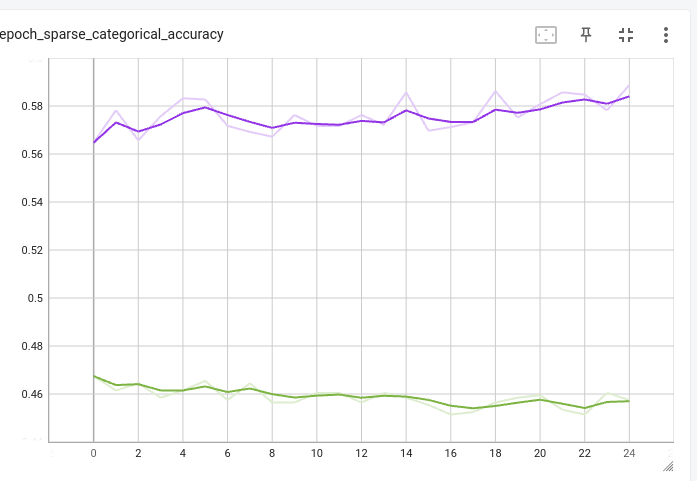
\includegraphics[height=1.5in]{screen11.png}
\end{center}
\end{frame}

\begin{frame}{TensorBoard}
\centering
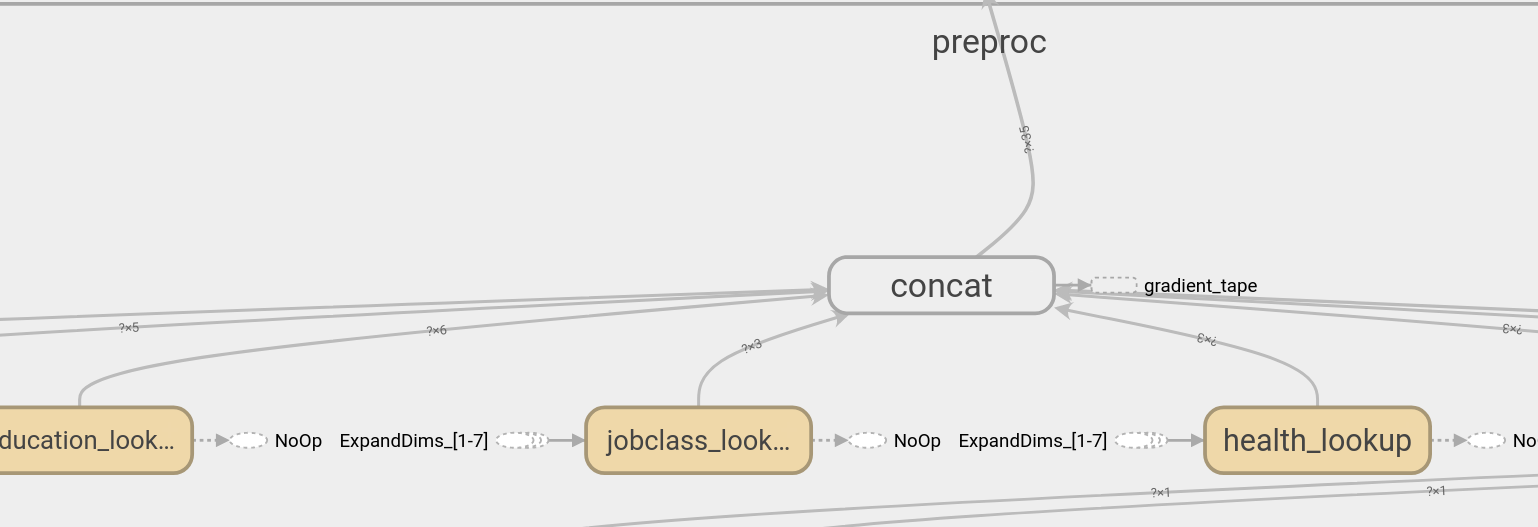
\includegraphics[width=.8\textwidth]{screen10.png} \\
\vspace{\baselineskip}
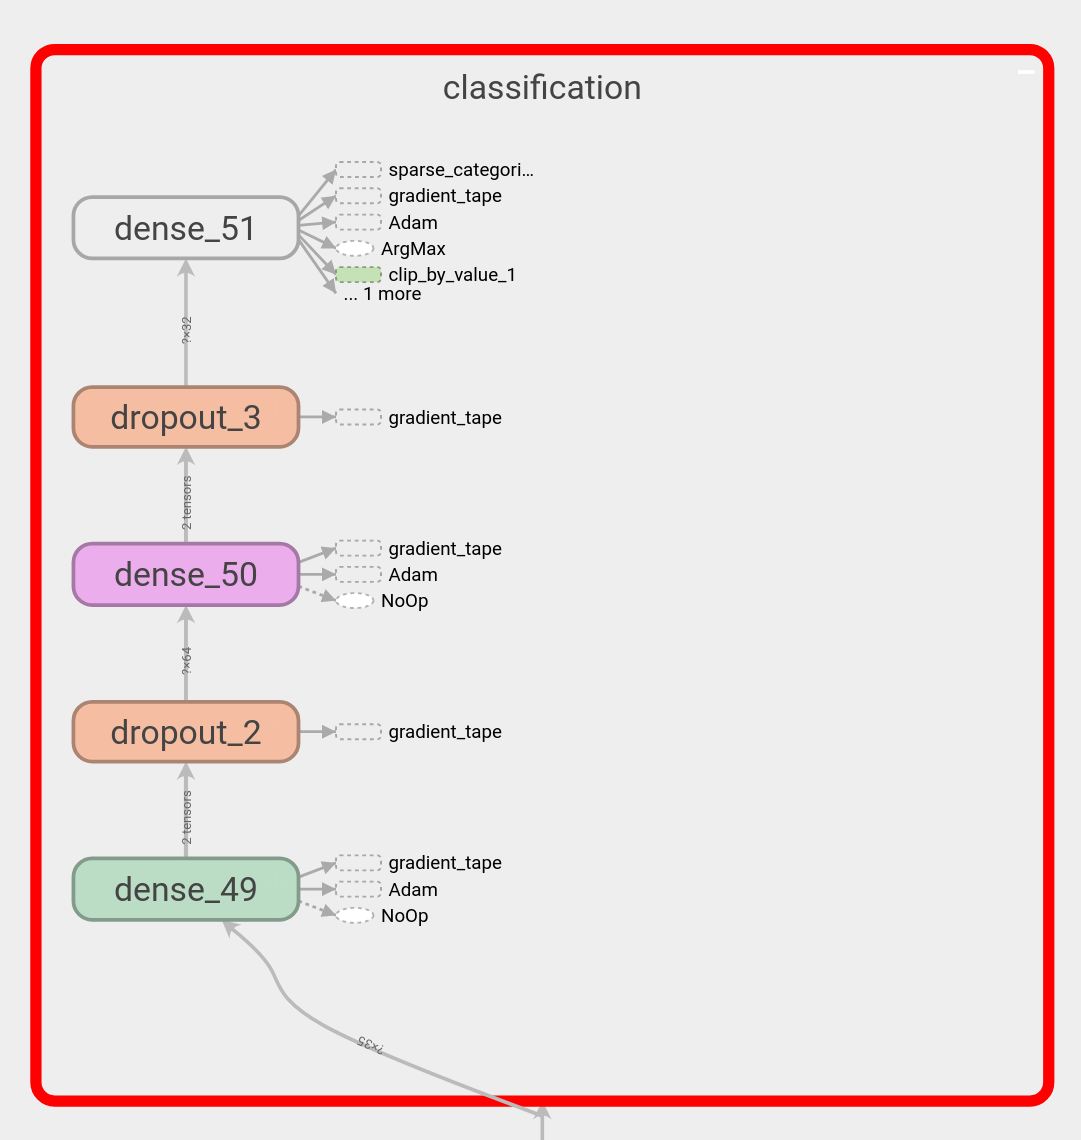
\includegraphics[height=2in]{screen9.png}
\end{frame}

\begin{frame}[fragile]{Early Stopping}
Another useful callback function:

\begin{pythoncode}
earlystop_callback = tf.keras.callbacks.EarlyStopping(
    monitor = 'val_loss',
    patience = 3,
    mode = 'min', 
    # or 'max' or 'auto' depending on monitor metric
    restore_best_weights = True)
\end{pythoncode}
\end{frame}


\begin{frame}{Hands-On Exercises}
\begin{itemize}
   \item Examine the model summaries for the pre-processing, the classification, and the complete wage model. Explain the number of trainable and total parameters, and also explain the output shapes of each layer.
   \item Make the ''wage'' prediction a binary classification problem:
   \begin{enumerate}
      \item Modify the \texttt{wage\_labels} and combine classes 0, 1 and classes 2, 3 (class numbers should be 0 or 1)
      \item Modify the classification network to have a single output node
      \item Use the \texttt{BinaryCrossentropy} loss
      \item Return the following metrics as part of the training history:
      \begin{itemize}
          \item Precision
          \item Recall
          \item AUC
      \end{itemize}
      \item Plot the metrics after training
   \end{enumerate}
\end{itemize}
\end{frame}

\end{document}



